\documentclass[10pt,a4paper]{article}

% -------------------- Packages --------------------
\usepackage[utf8]{inputenc}
\usepackage[T1]{fontenc}
\usepackage{lmodern}
\usepackage{microtype}
\usepackage{geometry}
\usepackage{amsmath,amssymb,amsfonts,bm}
\usepackage{graphicx}
\usepackage{booktabs}
\usepackage{array}
\usepackage{float}
\usepackage{caption}
\usepackage{subcaption}
\usepackage{dblfloatfix}
\usepackage{tabularx}
\usepackage{xcolor}
\usepackage{hyperref}
\usepackage{listings}
\usepackage{enumitem}
\usepackage{siunitx}
\usepackage{placeins}

% -------------------- Page setup --------------------
\geometry{top=1.7cm,bottom=1.8cm,left=1.55cm,right=1.55cm,columnsep=0.70cm}
\setlength{\parindent}{1.1em}
\setlength{\parskip}{0pt}
\graphicspath{{figures/}}
\sisetup{separate-uncertainty=true, exponent-product=\cdot}
\captionsetup{font=normalsize, labelfont=bf, justification=justified, singlelinecheck=false}
\renewcommand{\arraystretch}{1.08}
\renewcommand{\thesection}{\Roman{section}}
\renewcommand{\thesubsection}{\Alph{subsection}}
\renewcommand{\thesubsubsection}{\arabic{subsubsection}}
\definecolor{linkcolor}{rgb}{0,0,0.45}
\hypersetup{colorlinks=true, linkcolor=linkcolor, citecolor=linkcolor, urlcolor=linkcolor, breaklinks=true}
\pagestyle{plain}

\lstset{basicstyle=\ttfamily\footnotesize, breaklines=true, frame=single, columns=fullflexible, keepspaces=true, showstringspaces=false, backgroundcolor=\color{gray!5}}

% -------------------- Commands --------------------
\newcommand{\br}{\mathbf{r}}
\newcommand{\bR}{\mathbf{R}}
\newcommand{\dd}{\mathrm{d}}
\newcommand{\EL}{E_{\mathrm{L}}}
\newcommand{\code}[1]{\texttt{#1}}
\newcommand{\PsiT}{\Psi_{\mathrm{T}}}
\newcommand{\dt}{\Delta t}

\newcommand{\reportfigure}[3]{%
\begin{center}
\includegraphics[width=\columnwidth]{#1}
\captionof{figure}{#2}\label{#3}
\end{center}}

% -------------------- Title --------------------
\title{\vspace{-1.0cm}\Large FYS4411/FYS9411: Computational Physics II\\[0.35cm]
\Huge Variational Monte Carlo for Trapped Bosons\\[0.20cm]
\LARGE Project 1: harmonic traps, hard-sphere correlations, and one-body densities}
\author{Marius Torsheim\\Department of Physics, University of Oslo}
\date{Spring 2026}

\begin{document}
\twocolumn[
\begin{center}
{\large FYS4411/FYS9411: Computational Physics II\par}
\vspace{0.25cm}
{\LARGE\bfseries Variational Monte Carlo for Trapped Bosons\par}
\vspace{0.12cm}
{\large Project 1: harmonic traps, hard-sphere correlations, and one-body densities\par}
\vspace{0.35cm}
{Marius Torsheim\\Department of Physics, University of Oslo\par}
\vspace{0.15cm}
{Spring 2026\par}
\end{center}
\begin{center}
\textbf{Abstract}
\end{center}
\noindent
I implemented a variational Monte Carlo solver for a trapped Bose gas with a Gaussian one-body trial function and, in the interacting case, a hard-sphere Jastrow correlation factor. The non-interacting harmonic oscillator was used as the main validation problem because its exact energy is known analytically. Brute-force Metropolis calculations in one, two, and three dimensions reproduced the expected minima at $\alpha=0.5$, with $E/N=0.5$, $1.0$, and $1.5$, respectively. Importance sampling based on the Langevin equation was also implemented and showed the expected decrease in acceptance rate as the time step increased. A stochastic-gradient optimization of the variational parameter converged from $\alpha=0.7$ to $\alpha=0.5$ for $N=100$ particles in three dimensions, while the total energy converged to the exact value $E=150$. Blocking and bootstrap routines were added for statistical analysis of correlated Monte Carlo samples. Finally, the hard-core interaction with $a/a_{\mathrm{ho}}=0.0043$ was included in an anisotropic trap with $\beta=\gamma=2.82843$. The interacting energy per particle was larger than the ideal reference and increased with particle number, with minima near $\alpha=0.5$. The one-body density was only weakly changed by the short-range Jastrow factor for the parameters studied.
\vspace{0.30cm}
\begin{center}
Repository: \url{https://github.com/Torsheim/FYS4411_Project_1}
\end{center}
\vspace{0.55cm}
]

\section{Introduction}

Dilute trapped Bose gases provide a clean setting where many-body effects can be studied with controlled approximations. In the dilute regime the relevant two-body physics is largely determined by the $s$-wave scattering length, and the atoms can be modeled as hard spheres in a harmonic trap. Mean-field theory, through the Gross--Pitaevskii equation, is often accurate for small gas parameters, but Monte Carlo methods are useful when correlations become important or when one wants to benchmark mean-field approximations against explicitly correlated wave functions. The Project 1 task follows this strategy by building a variational Monte Carlo (VMC) solver first for a non-interacting harmonic oscillator, and then extending it to a hard-sphere Bose gas similar to the systems studied by DuBois and Glyde \cite{dubois2001} and by Nilsen \emph{et al.} \cite{nilsen2005}.

The aim of this work is twofold. First, I derive and implement the analytical local energy and drift force for the chosen trial state. Second, I validate the implementation against exact non-interacting harmonic-oscillator results before applying it to the repulsive hard-core problem. This separation is important: the non-interacting problem tests the sampler, local energy, variational parameter, optimization routine, and statistical analysis in a setting where the correct answer is known.

The report is organized as follows. Section~\ref{sec:theory} gives the Hamiltonian, trial wave function, local energy, drift force, and statistical estimators. Section~\ref{sec:methodology} describes the algorithms and implementation. Section~\ref{sec:results} presents the numerical results for parts 1b--1h. Section~\ref{sec:conclusion} summarizes the conclusions and discusses limitations. Appendix~\ref{app:reproducibility} gives the main run commands and code structure.

\section{Theory}\label{sec:theory}

\subsection{Hamiltonian and units}

Natural oscillator units are used throughout: $\hbar=m=\omega_{\perp}=1$. For the spherical, non-interacting harmonic oscillator in $d$ dimensions, the Hamiltonian is
\begin{equation}
    \hat{H}_0=\sum_{i=1}^{N}\frac{1}{2}\left(-\nabla_i^2+r_i^2\right).
    \label{eq:hamiltonian-spherical}
\end{equation}
For the anisotropic three-dimensional trap used in the interacting part, the dimensionless Hamiltonian becomes
\begin{equation}
    \hat{H}=\sum_{i=1}^{N}\frac{1}{2}\left(-\nabla_i^2+x_i^2+y_i^2+\gamma^2 z_i^2\right)
    +\sum_{i<j}V_{\mathrm{int}}(r_{ij}),
    \label{eq:hamiltonian-interacting}
\end{equation}
where $r_{ij}=|\br_i-\br_j|$ and
\begin{equation}
    V_{\mathrm{int}}(r_{ij})=
    \begin{cases}
    \infty, & r_{ij}\le a,\\
    0, & r_{ij}>a.
    \end{cases}
    \label{eq:hard-core}
\end{equation}
The trap anisotropy is
\begin{equation}
    \gamma=\frac{\omega_z}{\omega_{\perp}},
    \label{eq:gamma}
\end{equation}
and in the interacting calculations I use $\gamma=2.82843$ and $a/a_{\mathrm{ho}}=0.0043$, following the project specification.

\subsection{Trial wave function}

The trial wave function is
\begin{equation}
    \PsiT(\bR;\alpha,\beta)=
    \prod_{i=1}^{N}g(\br_i;\alpha,\beta)
    \prod_{j<k} f(r_{jk}),
    \label{eq:trial}
\end{equation}
where $\bR=(\br_1,\ldots,\br_N)$ and
\begin{equation}
    g(\br_i;\alpha,\beta)=\exp\left[-\alpha(x_i^2+y_i^2+\beta z_i^2)\right].
    \label{eq:gaussian}
\end{equation}
In one and two dimensions the obvious lower-dimensional forms are used. For spherical traps $\beta=1$. The Jastrow factor is
\begin{equation}
    f(r)=
    \begin{cases}
    0, & r\le a,\\
    1-a/r, & r>a.
    \end{cases}
    \label{eq:jastrow}
\end{equation}
In the implementation the logarithm of the wave function is used in most probability ratios. This avoids numerical underflow when the number of particles is large.

\subsection{Local energy for the ideal trap}

The local energy is
\begin{equation}
    \EL(\bR)=\frac{1}{\PsiT(\bR)}\hat{H}\PsiT(\bR).
    \label{eq:local-energy-def}
\end{equation}
For the non-interacting spherical oscillator, inserting $\PsiT=\exp(-\alpha\sum_i r_i^2)$ gives
\begin{equation}
    \EL(\bR)=\alpha dN+\left(\frac{1}{2}-2\alpha^2\right)\sum_{i=1}^{N}r_i^2.
    \label{eq:local-energy-nonint}
\end{equation}
The expectation value is
\begin{equation}
    \frac{\langle E\rangle}{N}=d\left(\frac{\alpha}{2}+\frac{1}{8\alpha}\right),
    \label{eq:variational-energy-nonint}
\end{equation}
which has its minimum at $\alpha=1/2$ and gives the exact ground-state energy $E/N=d/2$.

The drift force used in importance sampling is
\begin{equation}
    \mathbf{F}_i=2\frac{\nabla_i\PsiT}{\PsiT}=2\nabla_i\ln\PsiT.
    \label{eq:drift-force}
\end{equation}
For the non-interacting spherical oscillator this reduces to
\begin{equation}
    \mathbf{F}_i=-4\alpha\br_i.
    \label{eq:drift-nonint}
\end{equation}

\subsection{Jastrow derivatives}

For the interacting calculation I write the pair factor as $f(r)=\exp[u(r)]$ with
\begin{equation}
    u(r)=\ln(1-a/r),\qquad r>a.
\end{equation}
The first and second radial derivatives are
\begin{align}
    u'(r)&=\frac{a}{r(r-a)},\label{eq:uprime}\\
    u''(r)&=-\frac{a(2r-a)}{r^2(r-a)^2}.
    \label{eq:usecond}
\end{align}
For particle $k$,
\begin{equation}
    \nabla_k\ln\PsiT=\nabla_k\ln\phi(\br_k)+
    \sum_{j\ne k}\frac{\br_k-\br_j}{r_{kj}}u'(r_{kj}).
    \label{eq:grad-log-full}
\end{equation}
The interacting local energy is evaluated from
\begin{equation}
    \EL(\bR)=-\frac{1}{2}\sum_{k=1}^{N}\frac{\nabla_k^2\PsiT}{\PsiT}+V_{\mathrm{ext}}(\bR),
    \label{eq:interacting-local-summary}
\end{equation}
with the hard-core interaction imposed through the boundary condition $\PsiT=0$ for $r_{ij}\le a$. The implemented expression is equivalent to the product-rule form derived in the assignment: it contains the Gaussian Laplacian, the Gaussian--Jastrow cross term, the squared Jastrow-gradient term, and the Jastrow Laplacian.

\subsection{Monte Carlo estimators}

The VMC energy estimate is the sample average of the local energy,
\begin{equation}
    \langle E\rangle \approx \frac{1}{M}\sum_{m=1}^{M}\EL(\bR_m),
    \label{eq:vmc-estimator}
\end{equation}
where the configurations are distributed according to $|\PsiT|^2$. The brute-force Metropolis proposal is symmetric, so the acceptance probability is
\begin{equation}
    A(\bR\rightarrow\bR')=\min\left(1,\frac{|\PsiT(\bR')|^2}{|\PsiT(\bR)|^2}\right).
    \label{eq:metropolis-acceptance}
\end{equation}
For importance sampling I use the Langevin proposal
\begin{equation}
    \br_i' = \br_i + D\mathbf{F}_i\dt + \sqrt{\dt}\,\bm{\eta},
    \label{eq:langevin}
\end{equation}
with $D=1/2$ and normally distributed $\bm{\eta}$. The Metropolis--Hastings ratio then includes the ratio of Green's functions associated with Eq.~\eqref{eq:langevin}.

The derivative of the variational energy with respect to $\alpha$ is estimated using
\begin{equation}
    \frac{\partial \langle E\rangle}{\partial \alpha}=2\left(\langle \EL O_{\alpha}\rangle-\langle\EL\rangle\langle O_{\alpha}\rangle\right),
    \label{eq:energy-gradient}
\end{equation}
where $O_{\alpha}=\partial \ln\PsiT/\partial\alpha$. The statistical errors are estimated both naively and with blocking, following the standard strategy for correlated Monte Carlo data \cite{flyvbjerg1989}.

\section{Methodology and implementation}\label{sec:methodology}

\subsection{Code structure}

The implementation is organized as a Python package, \code{fys4411\_project1}. The most important modules are:
\begin{itemize}[leftmargin=*]
    \item \code{wavefunction.py}: Gaussian and Jastrow wave functions, log wave functions, derivatives, and drift force;
    \item \code{local\_energy.py}: analytical and numerical local-energy routines;
    \item \code{samplers.py}: brute-force and importance-sampling VMC drivers;
    \item \code{optimization.py}: parameter scans and stochastic-gradient optimization;
    \item \code{statistics.py}: blocking and bootstrap analysis;
    \item \code{density.py}: one-body radial density histograms.
\end{itemize}
The calculation scripts are placed in \code{scripts/}. The repository also contains unit tests under \code{tests/}. Before the production runs, the test suite passed with 25 tests.

\subsection{Algorithms}

The brute-force sampler updates one particle at a time. This keeps the acceptance rate reasonable even for $N=500$. The importance sampler also uses particle-by-particle updates, but proposes moves using the drift force. The essential structure of the VMC code is:
\begin{lstlisting}
initialize positions R
for cycle in range(burn_in + cycles):
    for particle k in 1,...,N:
        propose R' using brute-force or Langevin move
        compute Metropolis-Hastings acceptance ratio
        accept or reject the proposed move
    if cycle >= burn_in:
        store local energy and optional observables
return mean energy, variance, error, acceptance rate
\end{lstlisting}
For the optimization part, each iteration runs a VMC calculation at the current $\alpha$, estimates Eq.~\eqref{eq:energy-gradient}, and updates
\begin{equation}
    \alpha_{n+1}=\alpha_n-\eta\frac{\partial\langle E\rangle}{\partial\alpha}.
\end{equation}
A learning rate of $\eta=0.001$ was necessary for stable convergence for $N=100$ in three dimensions. Larger learning rates caused the parameter to bounce between the allowed bounds.

\subsection{Run parameters}

The non-interacting brute-force scan used $\alpha\in[0.3,0.7]$ with nine equally spaced values, $N=1,10,100,500$, dimensions $d=1,2,3$, 50000 production cycles, and 5000 burn-in cycles. Importance-sampling time-step studies used $\dt\in\{0.001,0.005,0.01,0.05,0.1,0.2\}$ with $N=100$. I used both $\alpha=0.5$, which is the exact wave function, and $\alpha=0.45$, which gives a nonzero local-energy variance. The interacting calculation used $N=10,50,100$, $\alpha\in[0.35,0.65]$, $\beta=\gamma=2.82843$, $a=0.0043$, 30000 production cycles, and 3000 burn-in cycles. The density calculation used $N=10$, $\alpha=0.5$, the same anisotropic trap parameters, and 50000 production cycles.

\section{Results and discussion}\label{sec:results}

\subsection{Non-interacting brute-force benchmarks}

The non-interacting harmonic oscillator is the most important benchmark because the exact solution is known. Figure~\ref{fig:partb} shows both the energy and the acceptance rate from the brute-force Metropolis scan. The energy curves have clear minima at $\alpha=0.5$ in all dimensions and for all particle numbers. At this value the local energy is constant and equal to the exact ground-state energy, explaining the zero variance seen in the output tables.

The acceptance rates also behave as expected. Increasing $\alpha$ narrows the wave function, so a fixed proposal step more often moves particles outside the high-probability region. The acceptance rate also decreases when going from one to three dimensions because a move changes more coordinates. The curves for different $N$ nearly overlap because the sampler updates one particle at a time.

\begin{figure*}[t]
\centering
\begin{subfigure}{0.32\textwidth}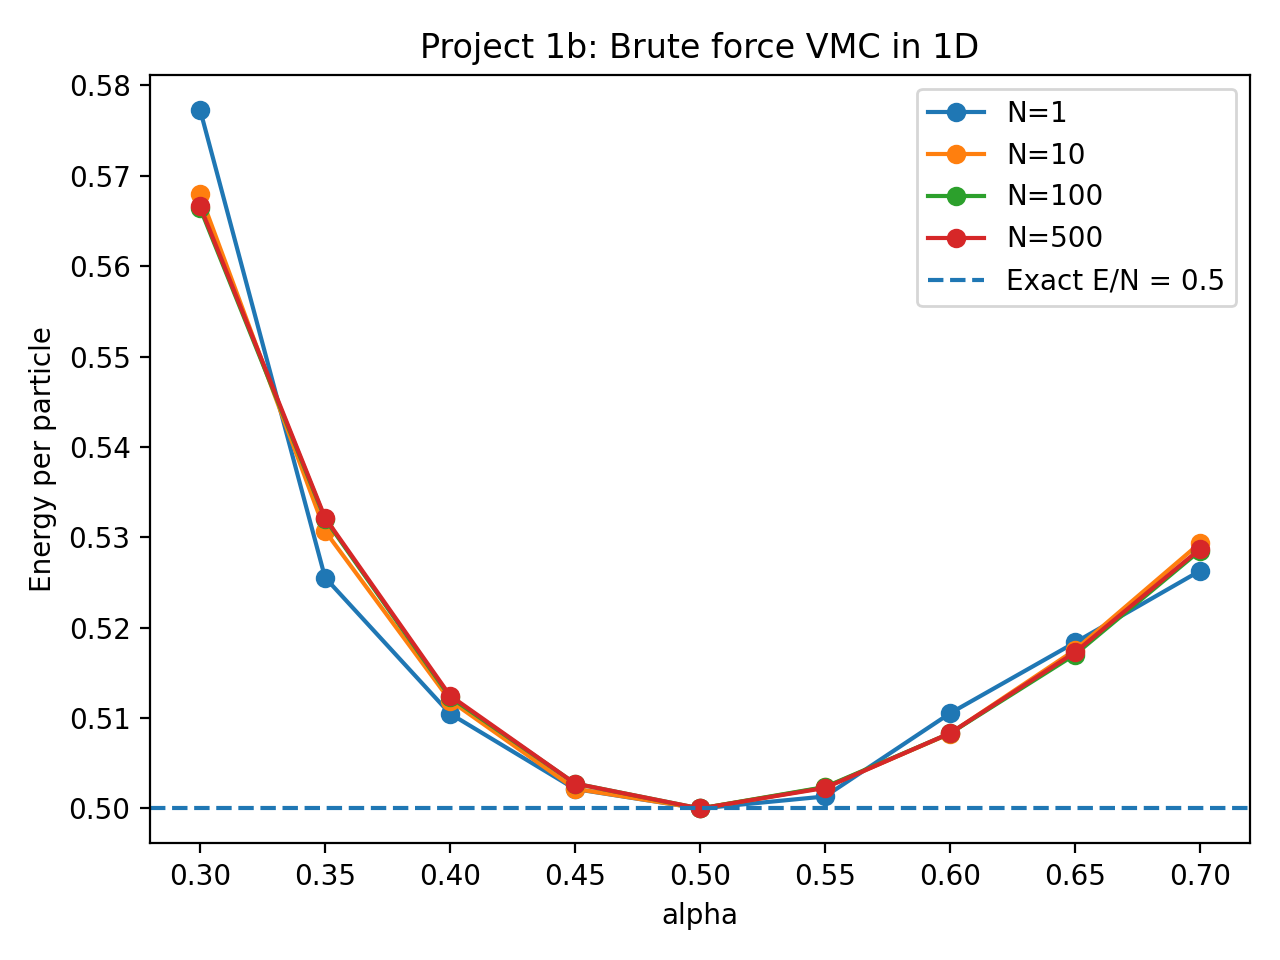
\includegraphics[width=\linewidth]{project1_b_energy_1D.png}\caption{Energy, 1D}\end{subfigure}
\begin{subfigure}{0.32\textwidth}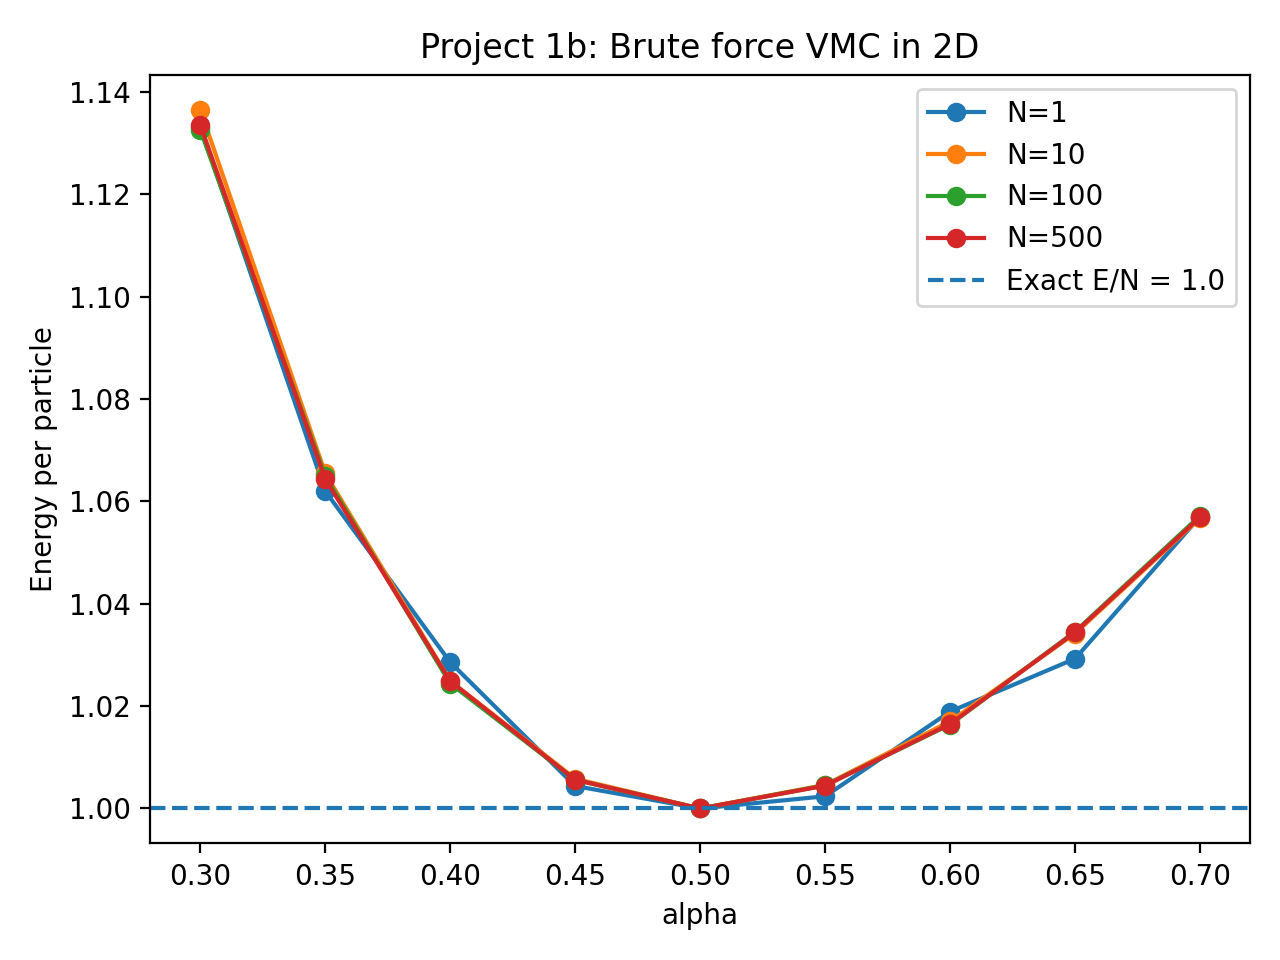
\includegraphics[width=\linewidth]{project1_b_energy_2D.png}\caption{Energy, 2D}\end{subfigure}
\begin{subfigure}{0.32\textwidth}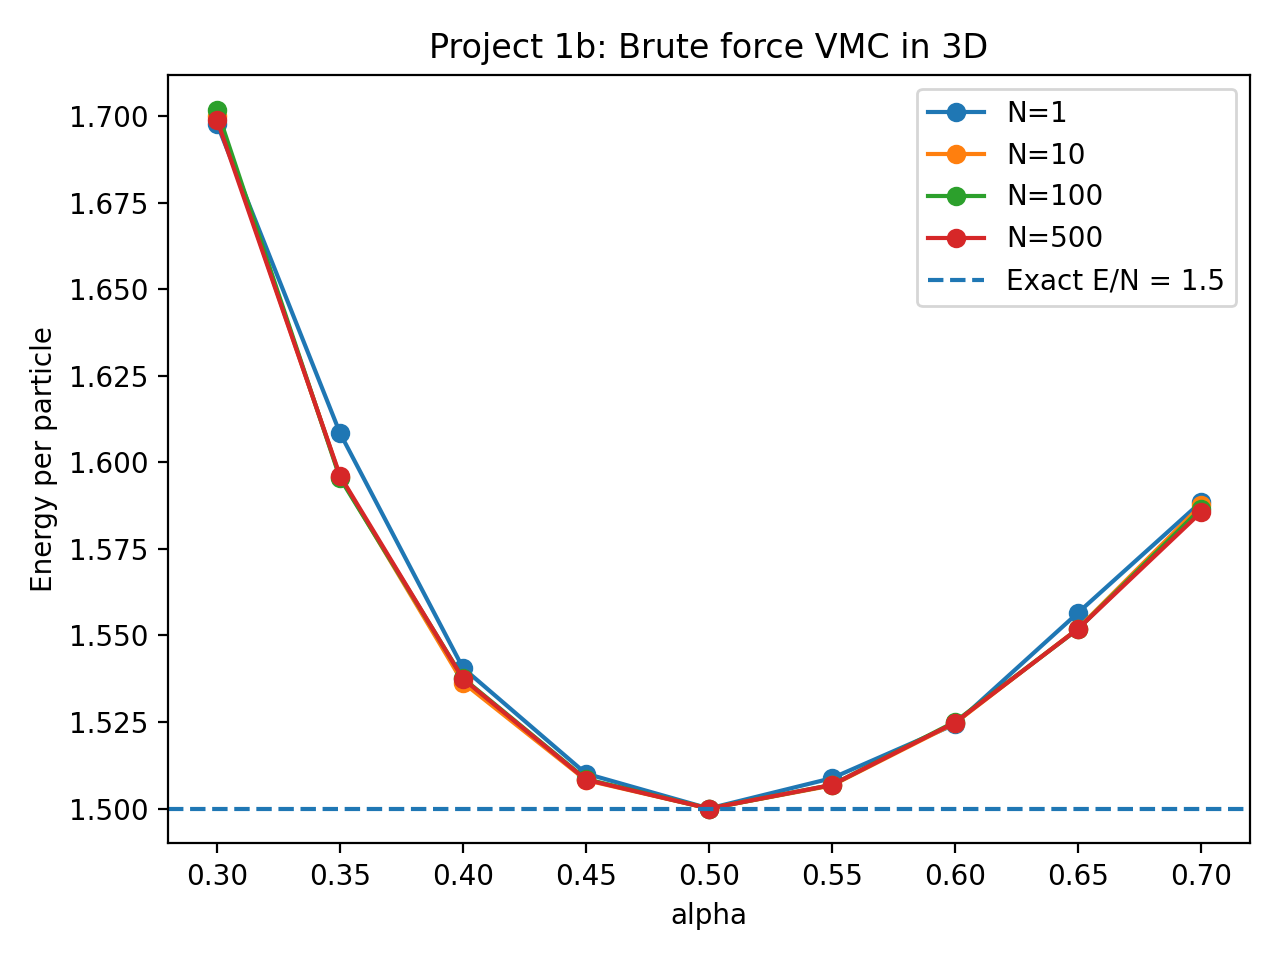
\includegraphics[width=\linewidth]{project1_b_energy_3D.png}\caption{Energy, 3D}\end{subfigure}
\begin{subfigure}{0.32\textwidth}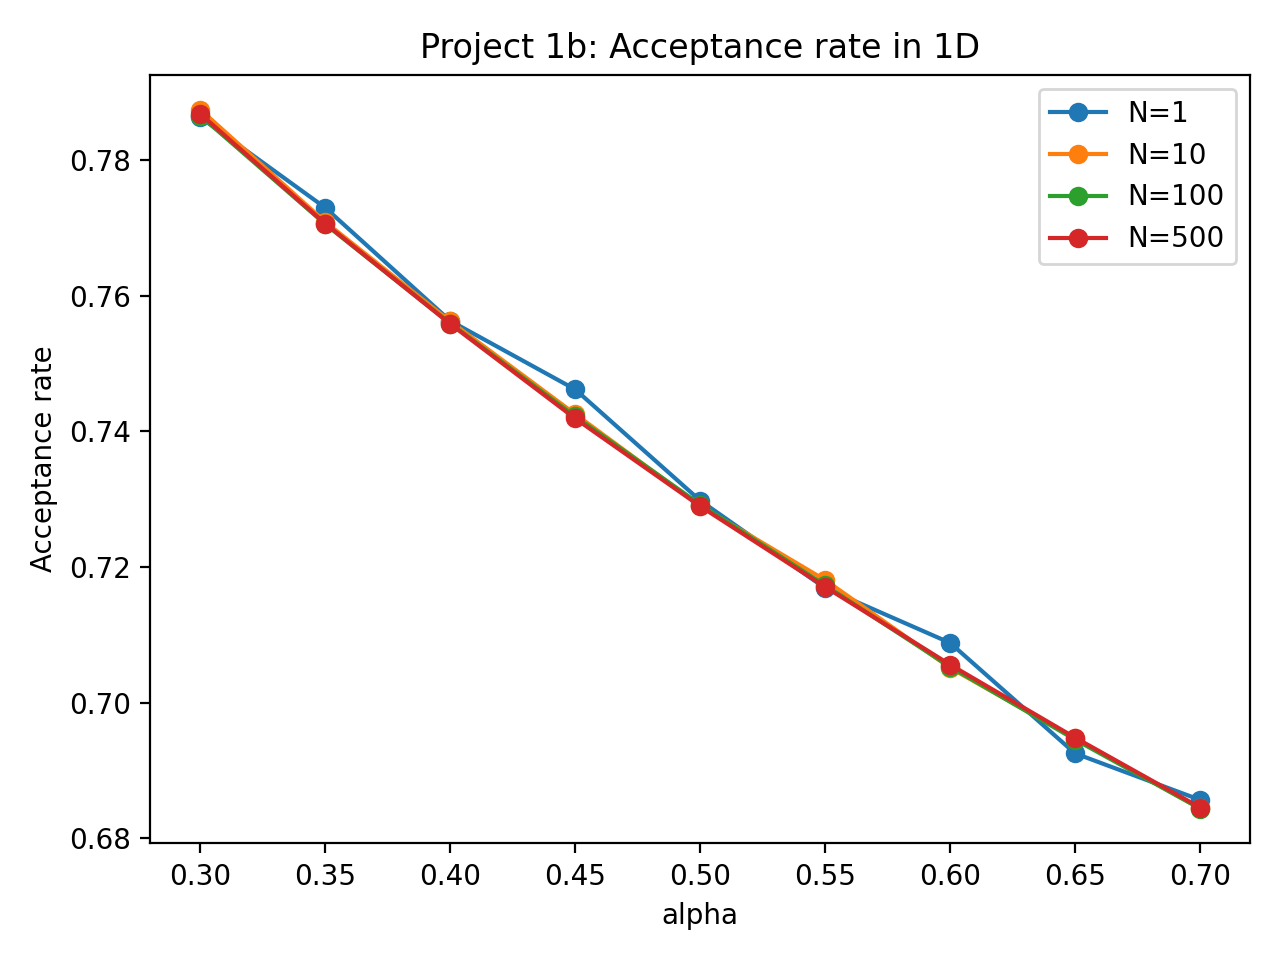
\includegraphics[width=\linewidth]{project1_b_acceptance_1D.png}\caption{Acceptance, 1D}\end{subfigure}
\begin{subfigure}{0.32\textwidth}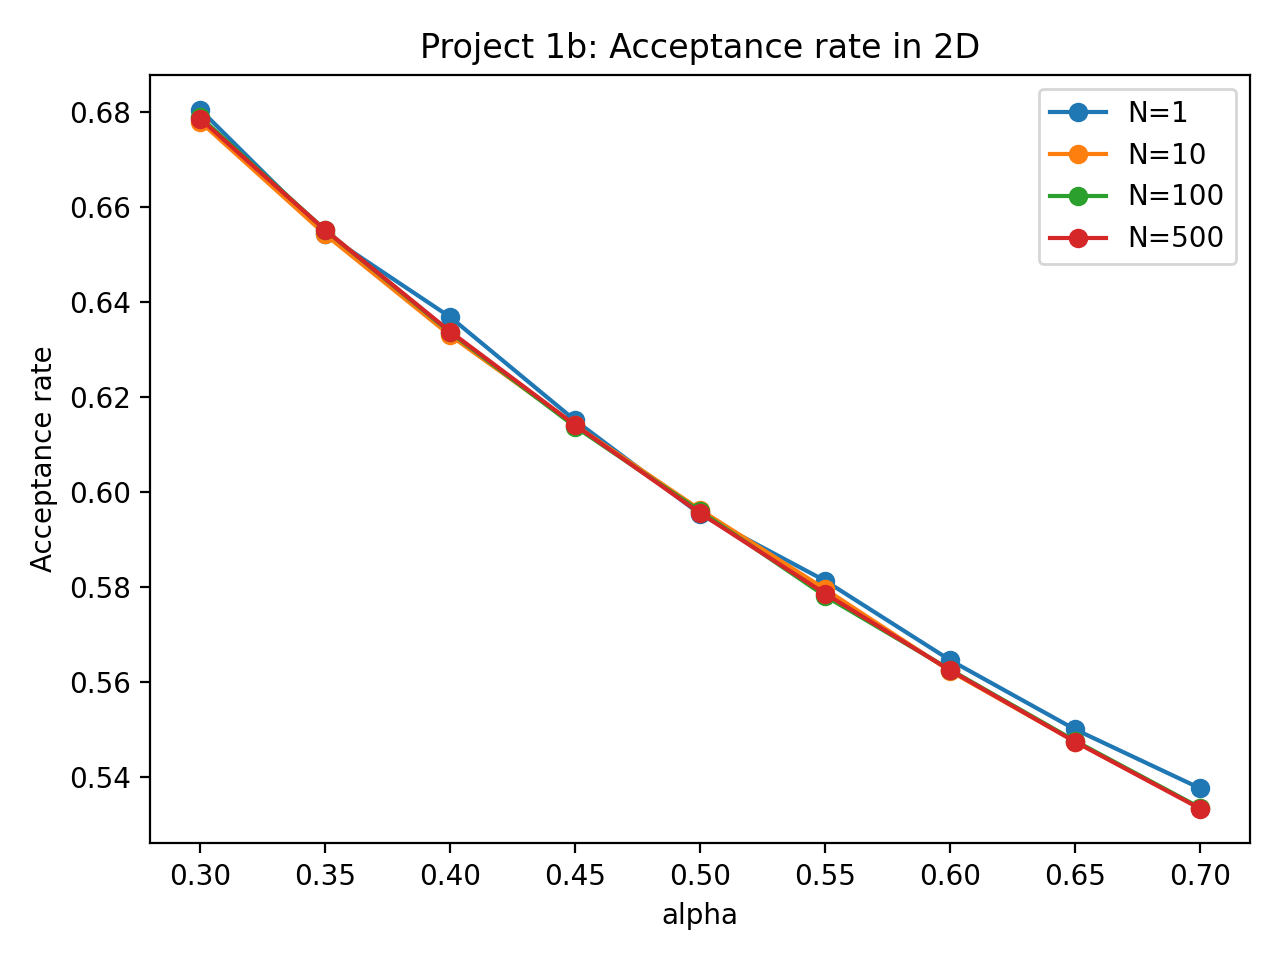
\includegraphics[width=\linewidth]{project1_b_acceptance_2D.png}\caption{Acceptance, 2D}\end{subfigure}
\begin{subfigure}{0.32\textwidth}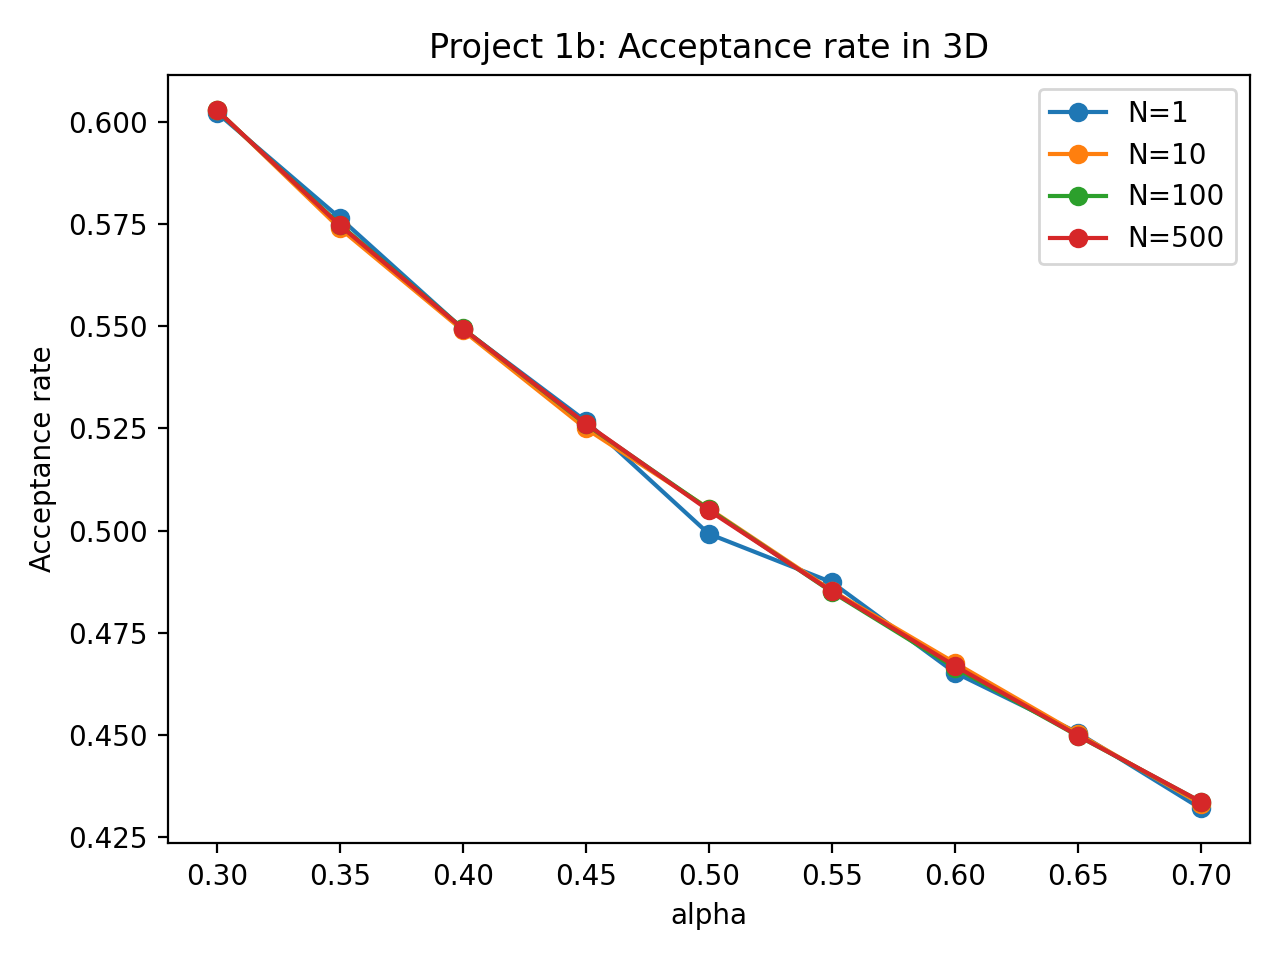
\includegraphics[width=\linewidth]{project1_b_acceptance_3D.png}\caption{Acceptance, 3D}\end{subfigure}
\caption{Project 1b brute-force Metropolis validation for the non-interacting harmonic oscillator. The energy per particle has its minimum at $\alpha=0.5$, where the exact values are $E/N=0.5$, $1.0$, and $1.5$ in one, two, and three dimensions. The acceptance rate decreases with both $\alpha$ and dimensionality.}
\label{fig:partb}
\end{figure*}

\begin{center}
\captionof{table}{Analytical reference values for the non-interacting oscillator at the optimal parameter $\alpha=0.5$. These values are independent of $N$ when reported per particle.}
\label{tab:ideal-reference}
\begin{tabular}{@{}ccc@{}}
\toprule
Dimension & $E/N$ & Exact optimum \\
\midrule
1D & 0.5 & $\alpha=0.5$\\
2D & 1.0 & $\alpha=0.5$\\
3D & 1.5 & $\alpha=0.5$\\
\bottomrule
\end{tabular}
\end{center}

\subsection{Importance sampling}

Importance sampling was tested by varying the Langevin time step. Figure~\ref{fig:partc-exact} shows the validation run at $\alpha=0.5$. Since this is the exact trial wave function for the ideal oscillator, the local energy is constant. The flat energy curves are therefore not a numerical accident; they show that the analytical local energy and drift force are mutually consistent. The acceptance rate decreases smoothly as the time step increases, which is the expected behavior for Langevin proposals.

\begin{figure*}[t]
\centering
\begin{subfigure}{0.32\textwidth}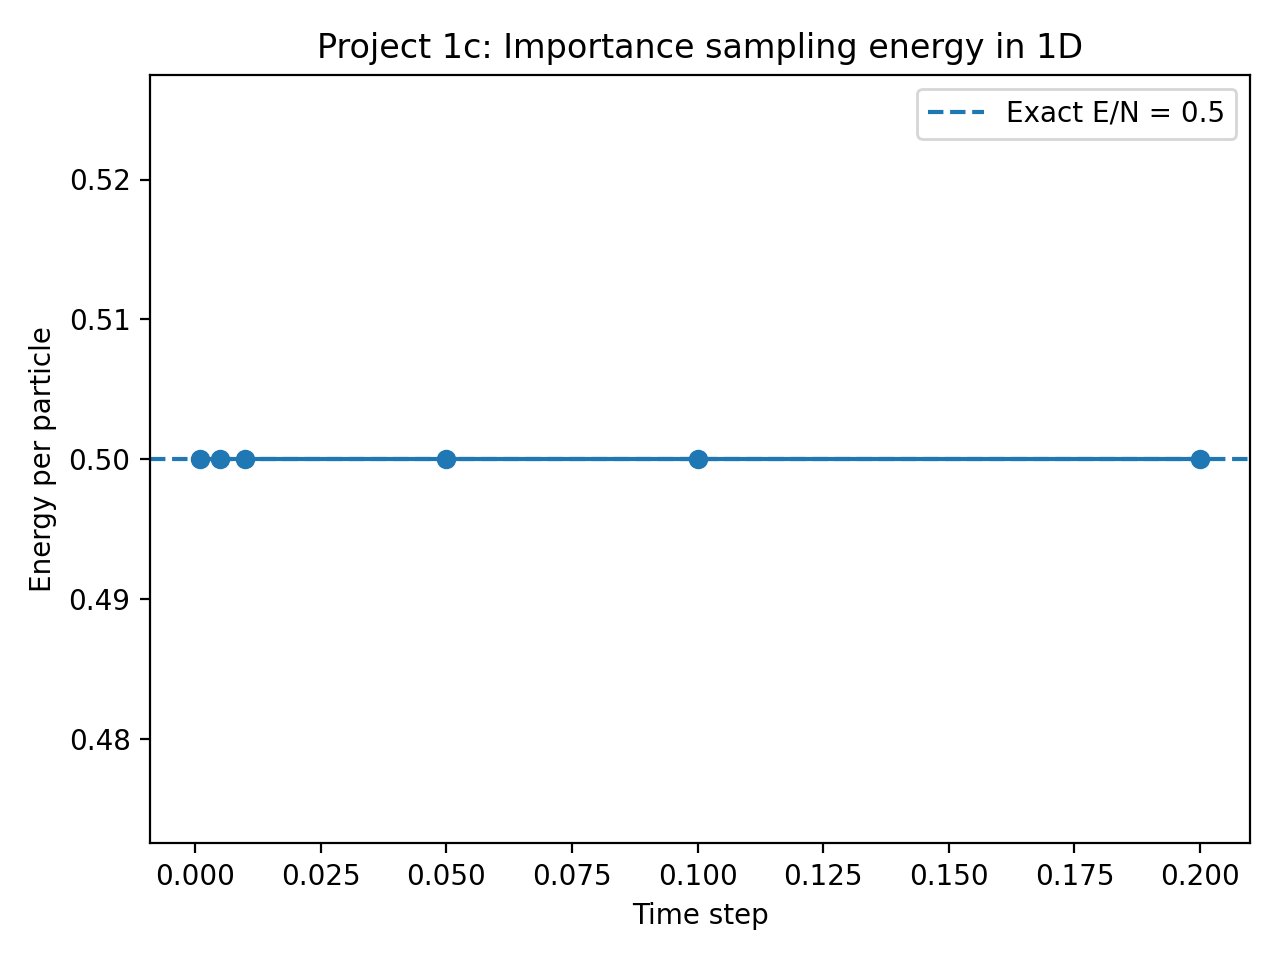
\includegraphics[width=\linewidth]{project1_c_energy_1D.png}\caption{Energy, 1D}\end{subfigure}
\begin{subfigure}{0.32\textwidth}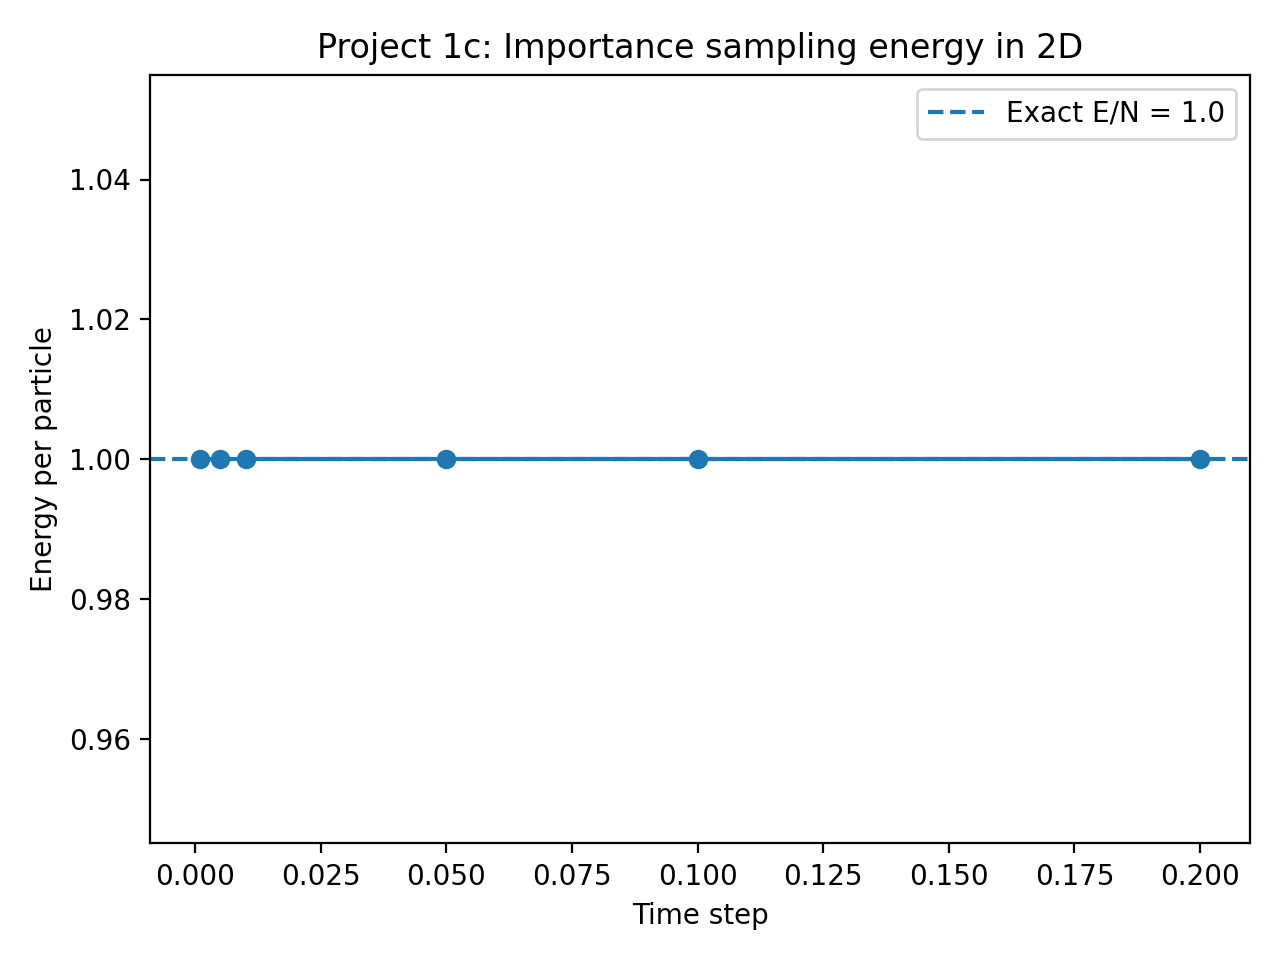
\includegraphics[width=\linewidth]{project1_c_energy_2D.png}\caption{Energy, 2D}\end{subfigure}
\begin{subfigure}{0.32\textwidth}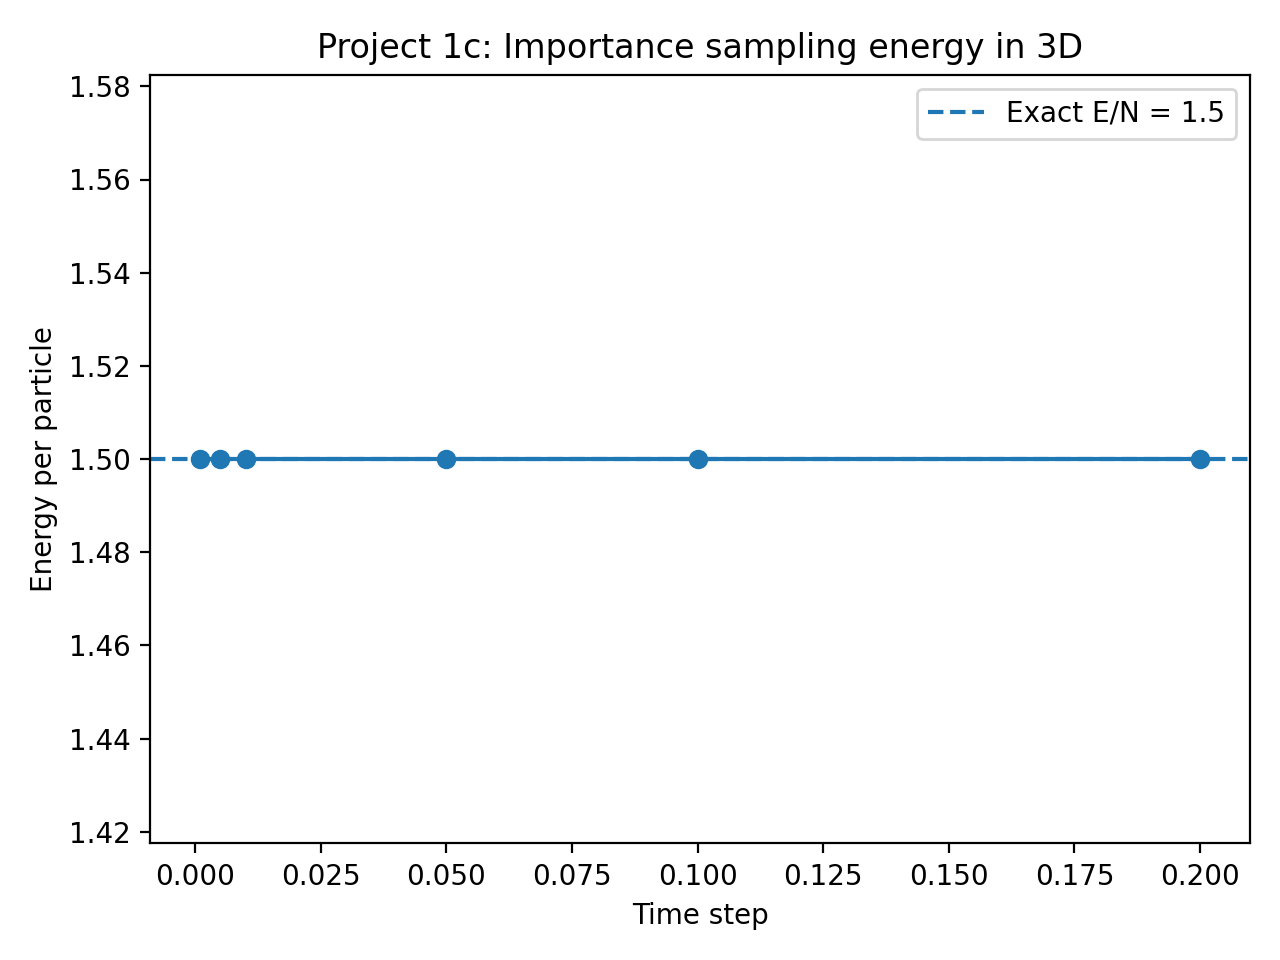
\includegraphics[width=\linewidth]{project1_c_energy_3D.png}\caption{Energy, 3D}\end{subfigure}
\begin{subfigure}{0.32\textwidth}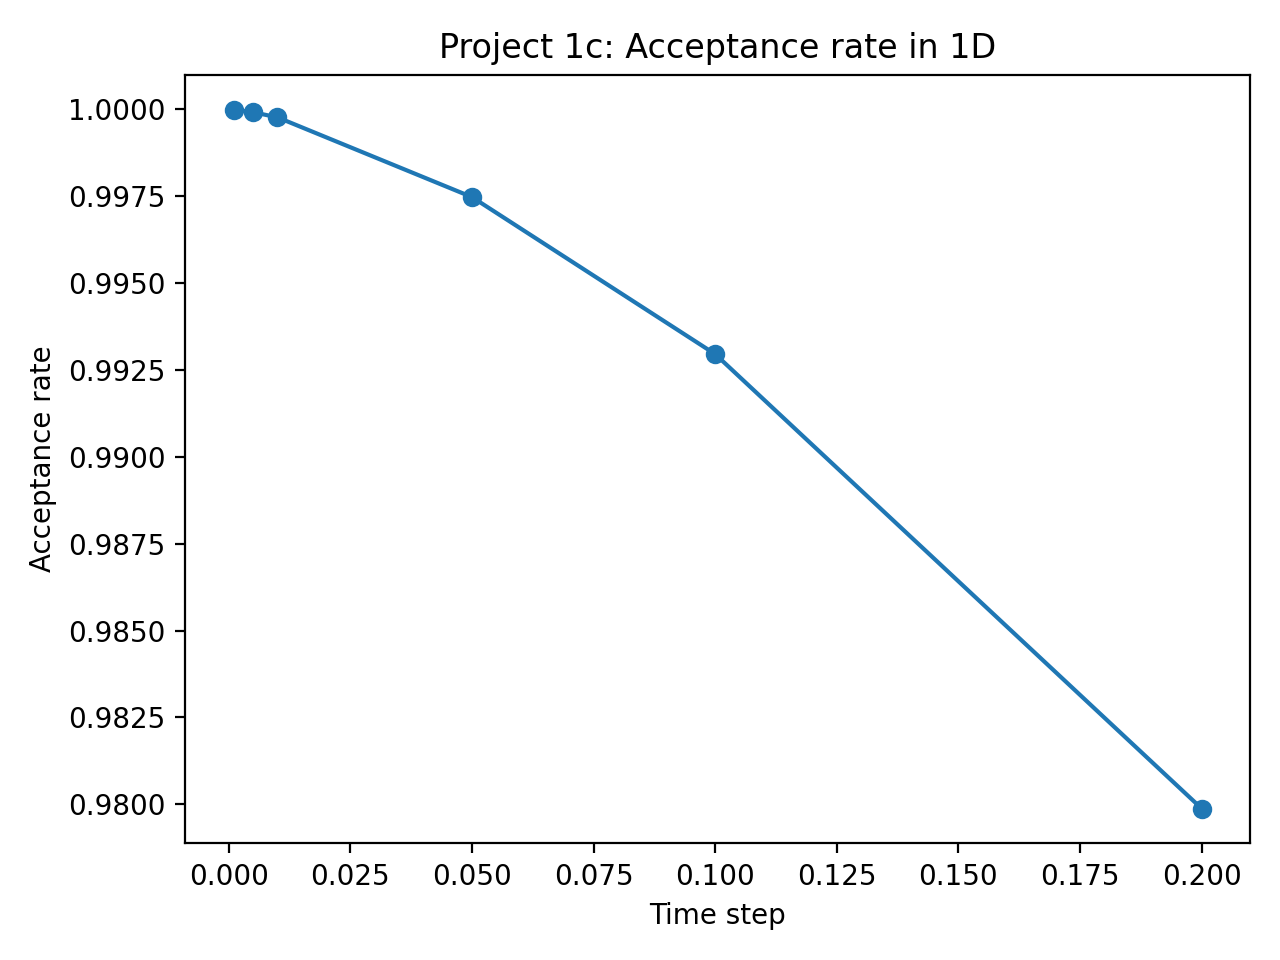
\includegraphics[width=\linewidth]{project1_c_acceptance_1D.png}\caption{Acceptance, 1D}\end{subfigure}
\begin{subfigure}{0.32\textwidth}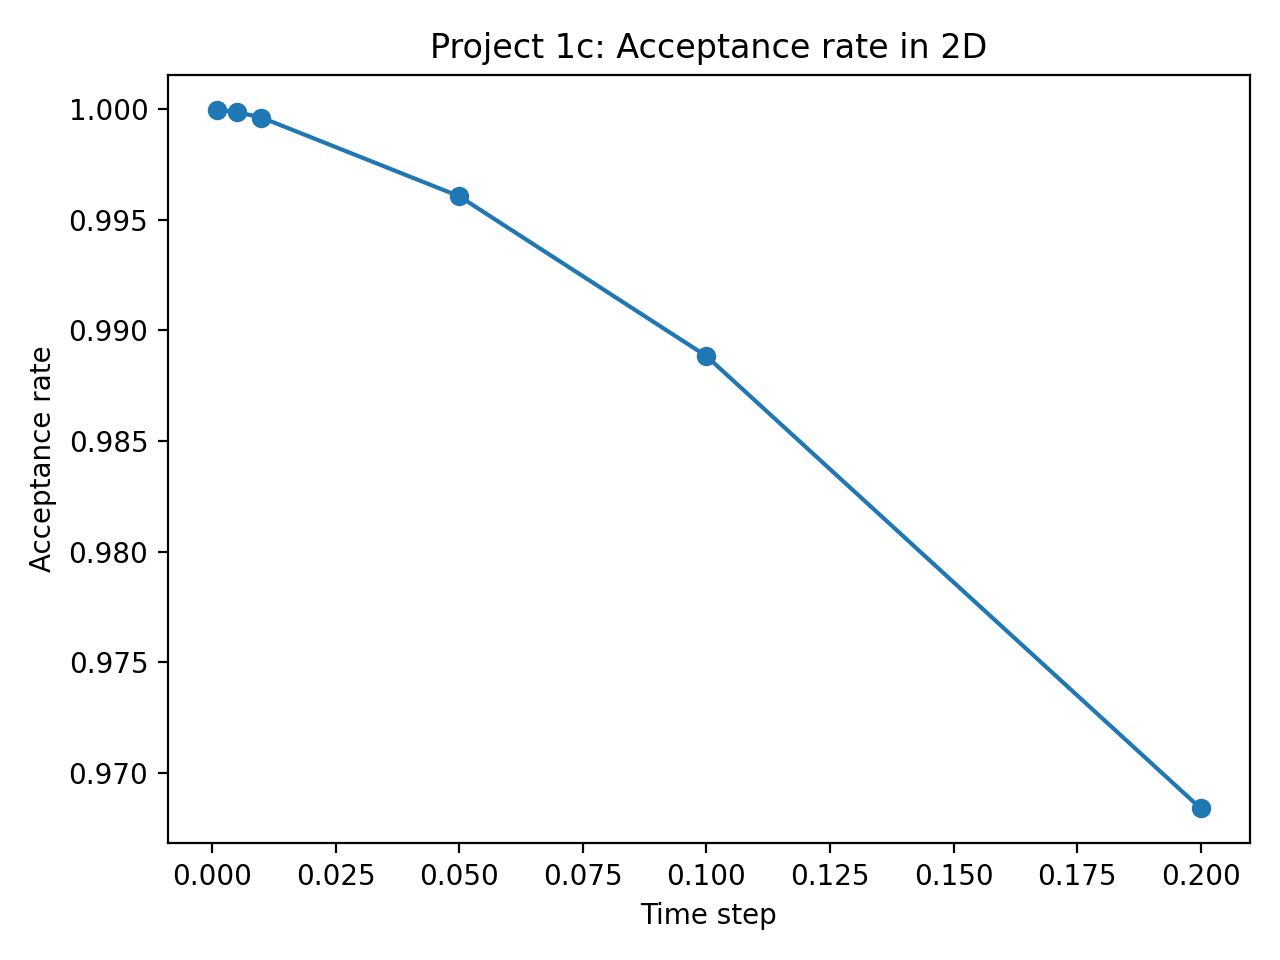
\includegraphics[width=\linewidth]{project1_c_acceptance_2D.png}\caption{Acceptance, 2D}\end{subfigure}
\begin{subfigure}{0.32\textwidth}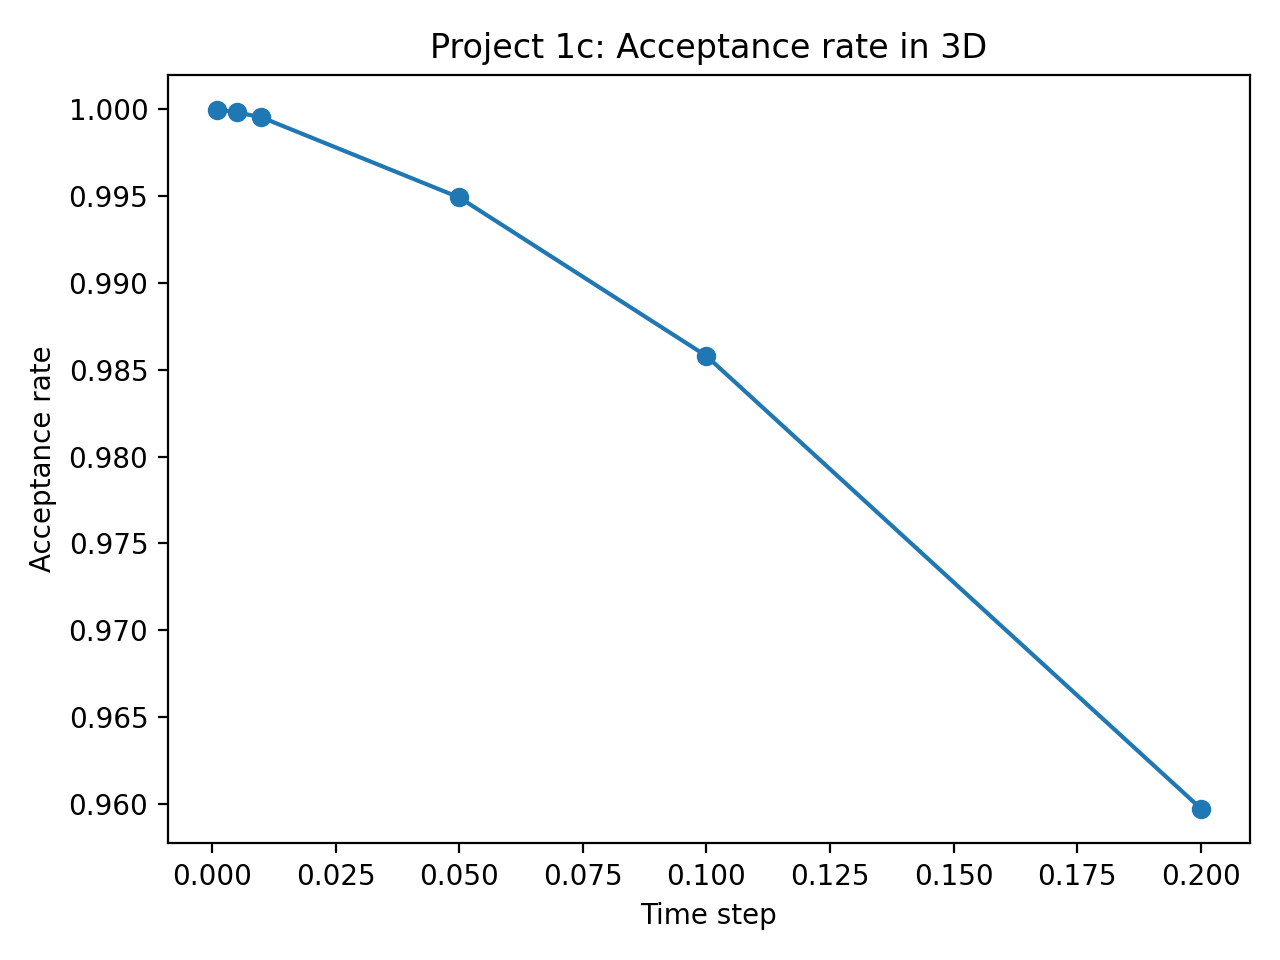
\includegraphics[width=\linewidth]{project1_c_acceptance_3D.png}\caption{Acceptance, 3D}\end{subfigure}
\caption{Project 1c importance-sampling validation at $\alpha=0.5$. The energy is exactly flat because the trial state is the exact ground-state wave function for the ideal trap. The acceptance rate decreases as the time step increases.}
\label{fig:partc-exact}
\end{figure*}

A second time-step study was made with $\alpha=0.45$, shown in Fig.~\ref{fig:partc-alpha045}. In this case the local energy has a finite variance, so the energy estimates fluctuate around the analytical variational energy from Eq.~\eqref{eq:variational-energy-nonint}. The deviations are small on the scale of the energy. The high acceptance rates indicate that all tested time steps are conservative for this simple problem, although the largest time step is beginning to show reduced acceptance.

\begin{figure*}[t]
\centering
\begin{subfigure}{0.32\textwidth}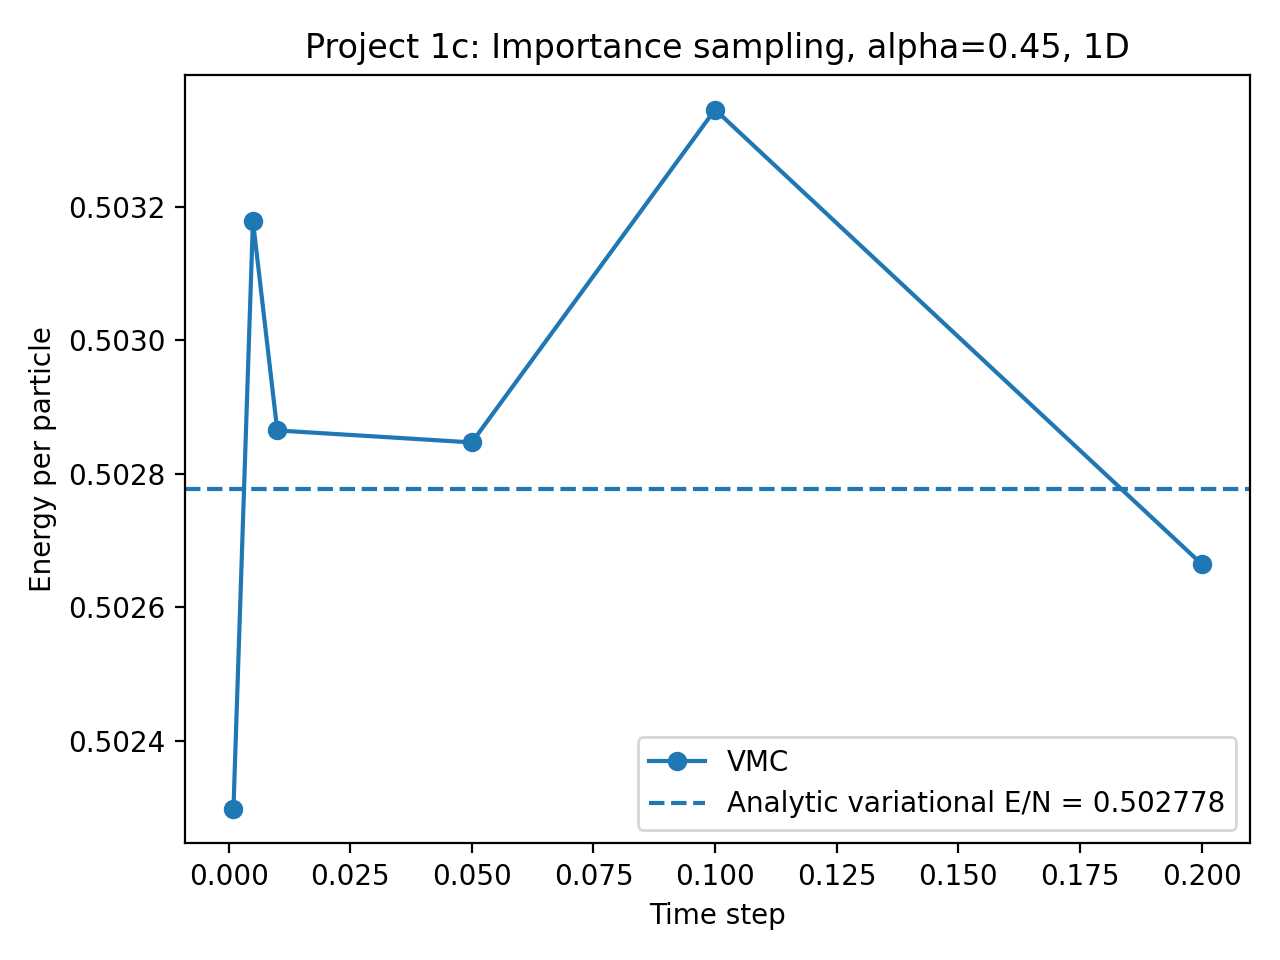
\includegraphics[width=\linewidth]{project1_c_alpha045_energy_1D.png}\caption{Energy, 1D}\end{subfigure}
\begin{subfigure}{0.32\textwidth}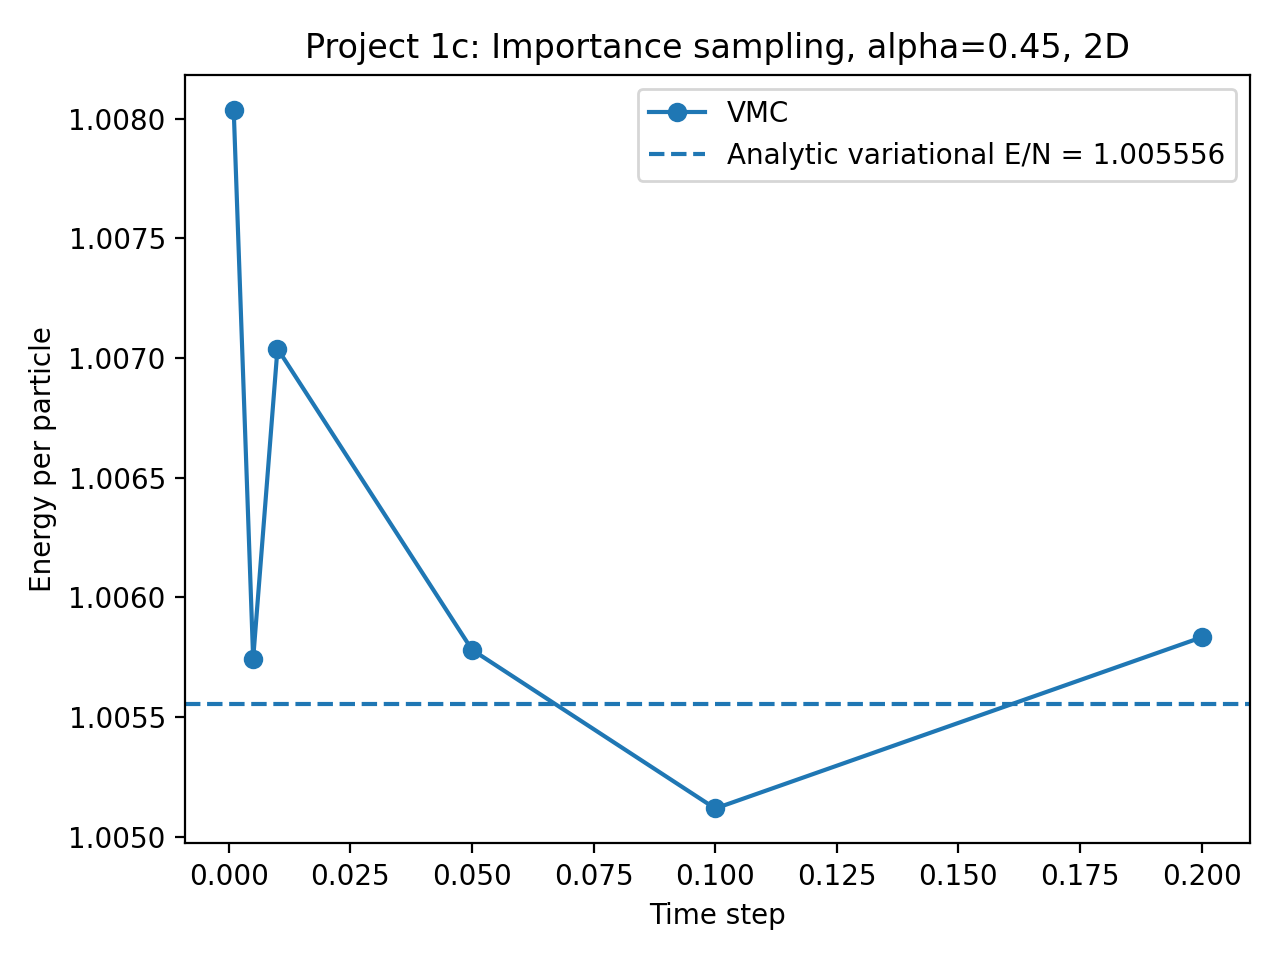
\includegraphics[width=\linewidth]{project1_c_alpha045_energy_2D.png}\caption{Energy, 2D}\end{subfigure}
\begin{subfigure}{0.32\textwidth}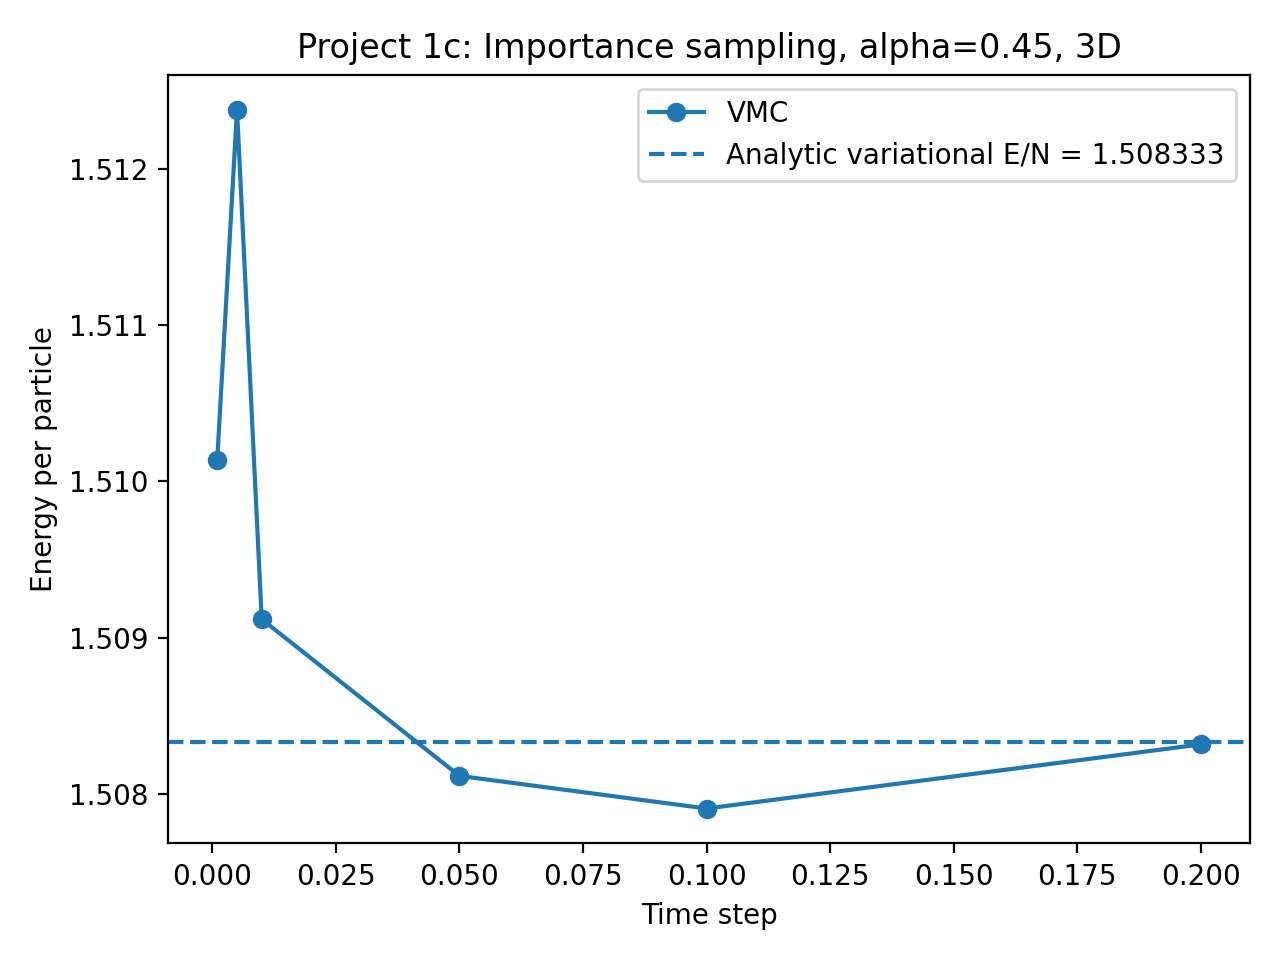
\includegraphics[width=\linewidth]{project1_c_alpha045_energy_3D.png}\caption{Energy, 3D}\end{subfigure}
\begin{subfigure}{0.32\textwidth}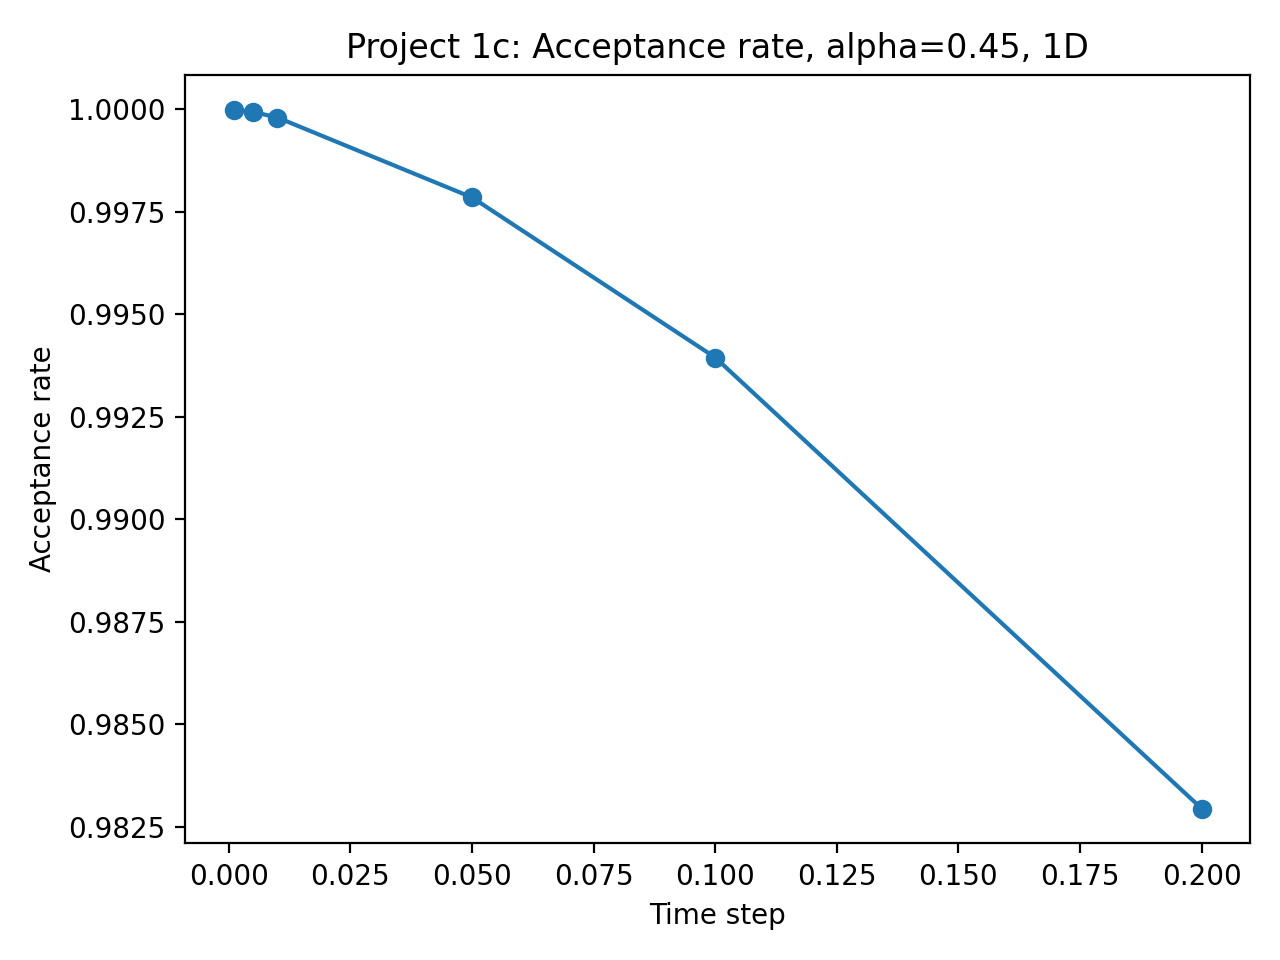
\includegraphics[width=\linewidth]{project1_c_alpha045_acceptance_1D.png}\caption{Acceptance, 1D}\end{subfigure}
\begin{subfigure}{0.32\textwidth}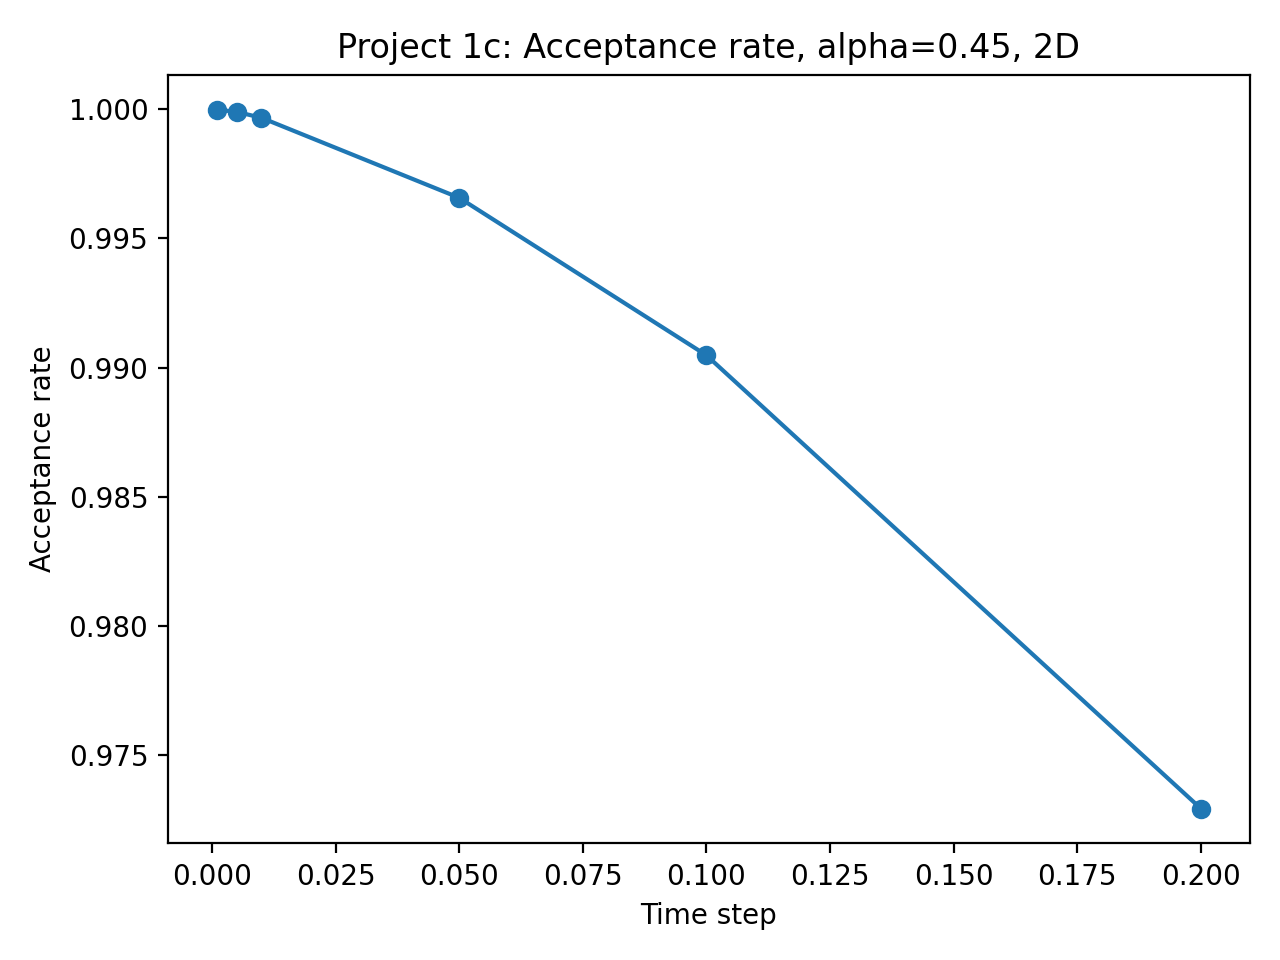
\includegraphics[width=\linewidth]{project1_c_alpha045_acceptance_2D.png}\caption{Acceptance, 2D}\end{subfigure}
\begin{subfigure}{0.32\textwidth}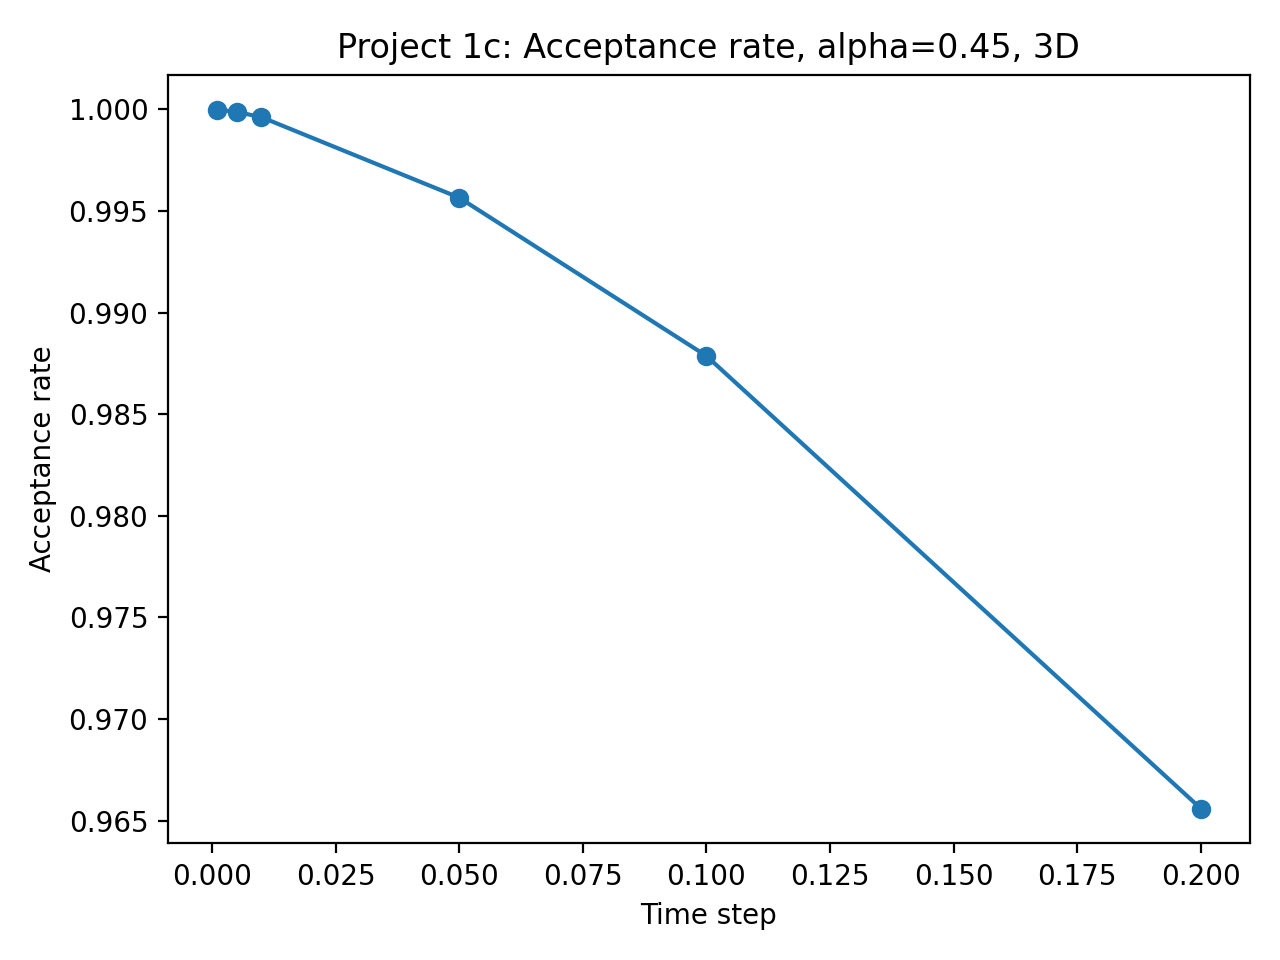
\includegraphics[width=\linewidth]{project1_c_alpha045_acceptance_3D.png}\caption{Acceptance, 3D}\end{subfigure}
\caption{Importance sampling at $\alpha=0.45$. The energy estimates fluctuate around the analytical variational values $E/N=0.502778$, $1.005556$, and $1.508333$ in one, two, and three dimensions. The fluctuations are Monte Carlo noise on a very narrow vertical scale.}
\label{fig:partc-alpha045}
\end{figure*}

\subsection{Optimization and statistical analysis}

Figure~\ref{fig:partd} shows the stochastic-gradient optimization of $\alpha$ for $N=100$ particles in three dimensions. Starting from $\alpha=0.7$, the parameter converges smoothly to $\alpha=0.5$. The total energy converges to $E=150$, which is the exact non-interacting ground-state energy for $N=100$ in three dimensions. The gradient magnitude decreases by many orders of magnitude, confirming that the optimization has reached the minimum.

\begin{figure*}[t]
\centering
\begin{subfigure}{0.32\textwidth}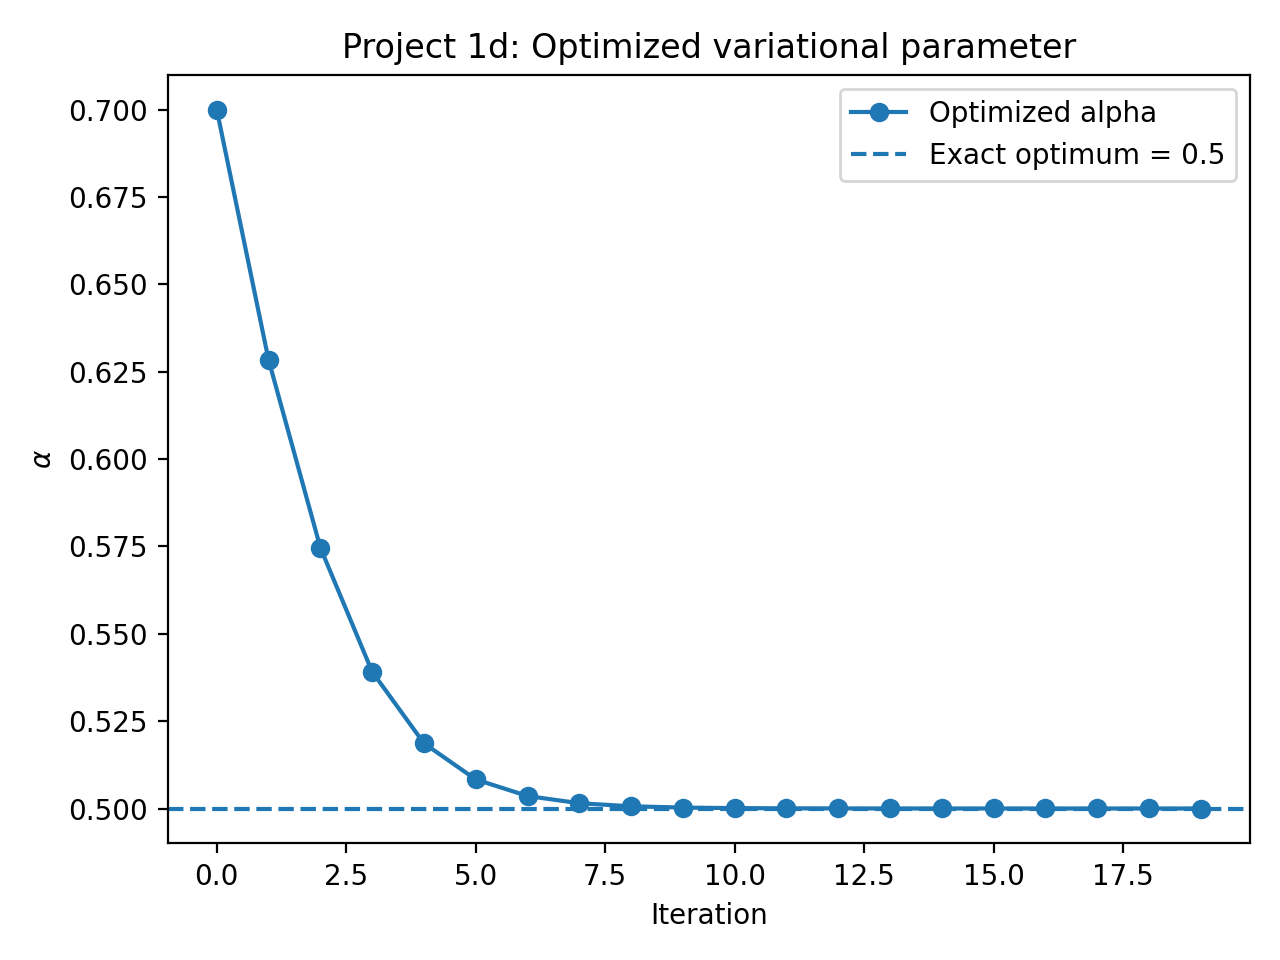
\includegraphics[width=\linewidth]{project1_d_CURRENT_alpha_vs_iteration.png}\caption{Optimized $\alpha$}\end{subfigure}
\begin{subfigure}{0.32\textwidth}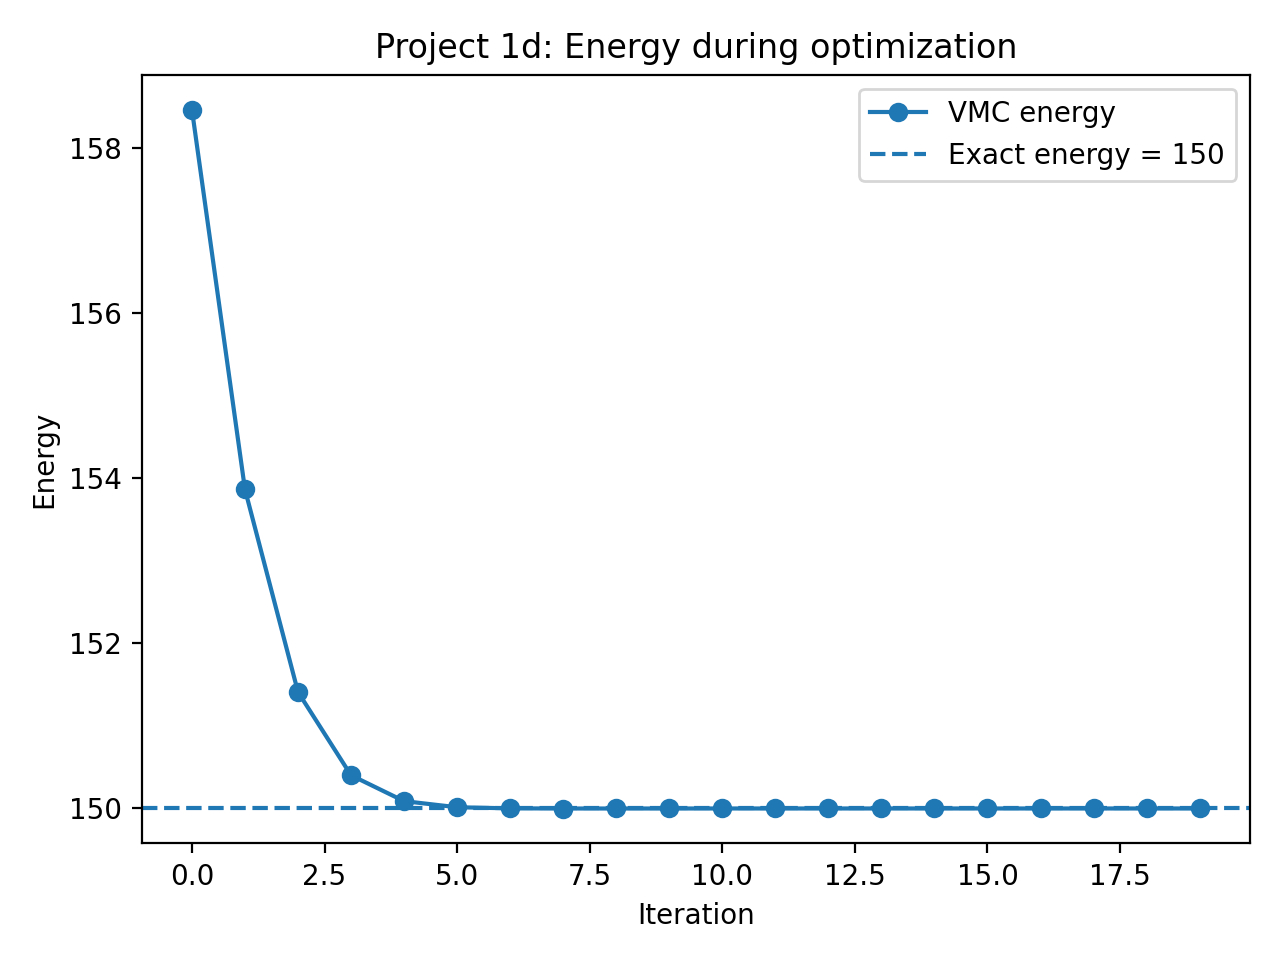
\includegraphics[width=\linewidth]{project1_d_CURRENT_energy_vs_iteration.png}\caption{Energy}\end{subfigure}
\begin{subfigure}{0.32\textwidth}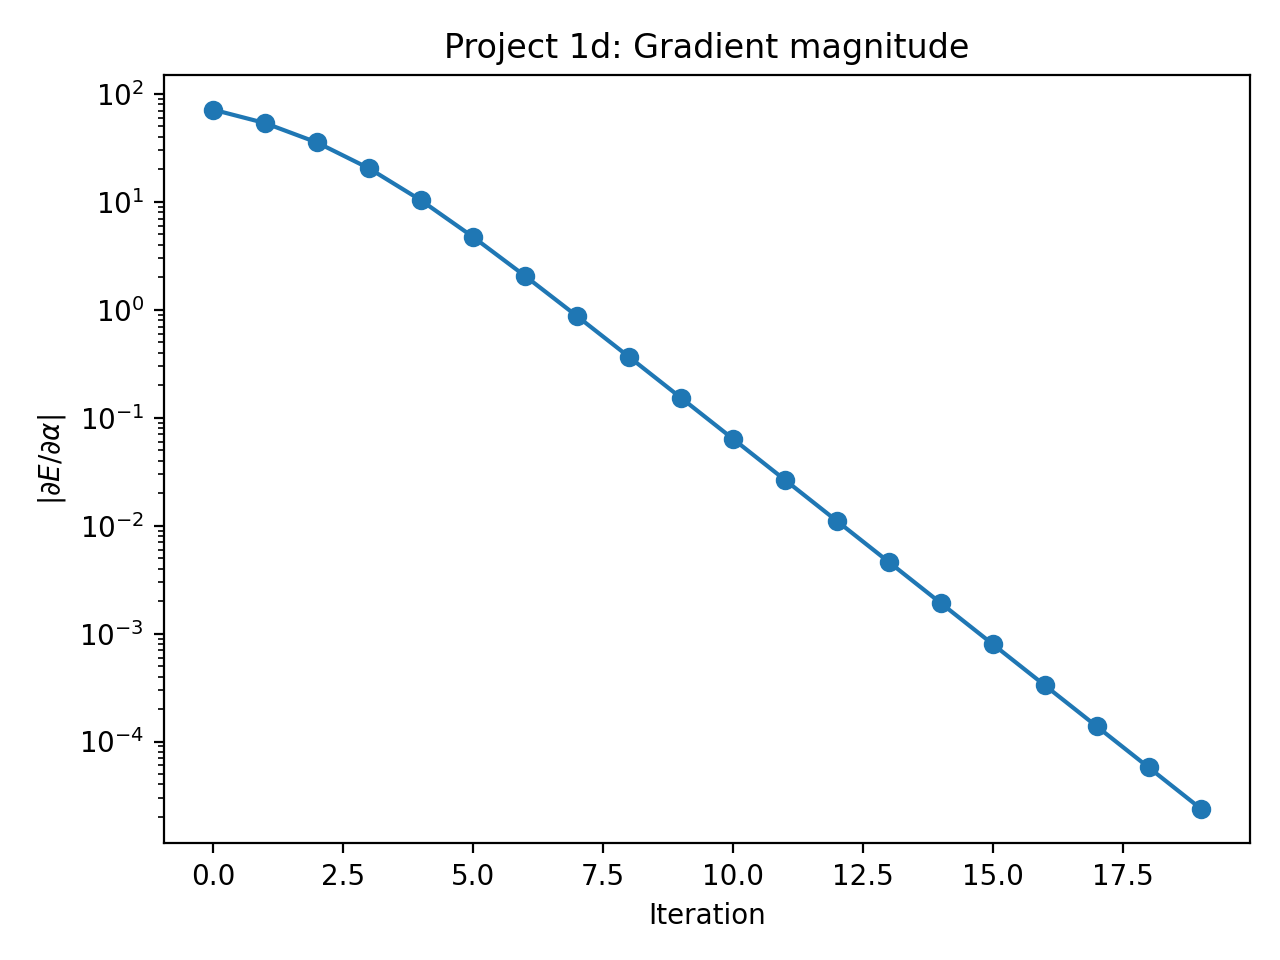
\includegraphics[width=\linewidth]{project1_d_CURRENT_gradient_vs_iteration.png}\caption{Gradient magnitude}\end{subfigure}
\caption{Project 1d stochastic-gradient optimization for $N=100$ particles in three dimensions. A learning rate of $0.001$ gives stable convergence to the analytical optimum $\alpha=0.5$ and energy $E=150$.}
\label{fig:partd}
\end{figure*}

The blocking analysis in Fig.~\ref{fig:parte} was performed at $\alpha=0.45$ to avoid the zero-variance special case at $\alpha=0.5$. The estimated standard error increases as correlated samples are grouped into larger blocks. This indicates that the naive unblocked error underestimates the uncertainty. The largest block sizes are themselves noisy because few blocks remain, so the best conservative error should be read from the broad middle-to-large block region rather than from the final point alone.

\reportfigure{project1_e_blocking_alpha045.png}{Project 1e blocking analysis for the non-interacting three-dimensional system at $\alpha=0.45$. The rise relative to the smallest block sizes shows the effect of autocorrelation in the local-energy samples.}{fig:parte}

\subsection{Hard-core repulsive interaction}

The hard-sphere interaction was included with $a/a_{\mathrm{ho}}=0.0043$ in an anisotropic trap with $\beta=\gamma=2.82843$. Figure~\ref{fig:partg} shows the energy per particle for $N=10$, $50$, and $100$. The orange reference line is the ideal non-interacting ground-state energy per particle in the same trap,
\begin{equation}
    \frac{E_0}{N}=\frac{1}{2}(2+\gamma)=2.414215.
\end{equation}
The interacting energies are all above this reference, as expected for a repulsive hard-core interaction. The minima remain close to $\alpha=0.5$, indicating that the one-body harmonic trap still largely controls the optimal Gaussian width, while the Jastrow factor handles most of the short-distance correlation.

\begin{figure*}[t]
\centering
\begin{subfigure}{0.32\textwidth}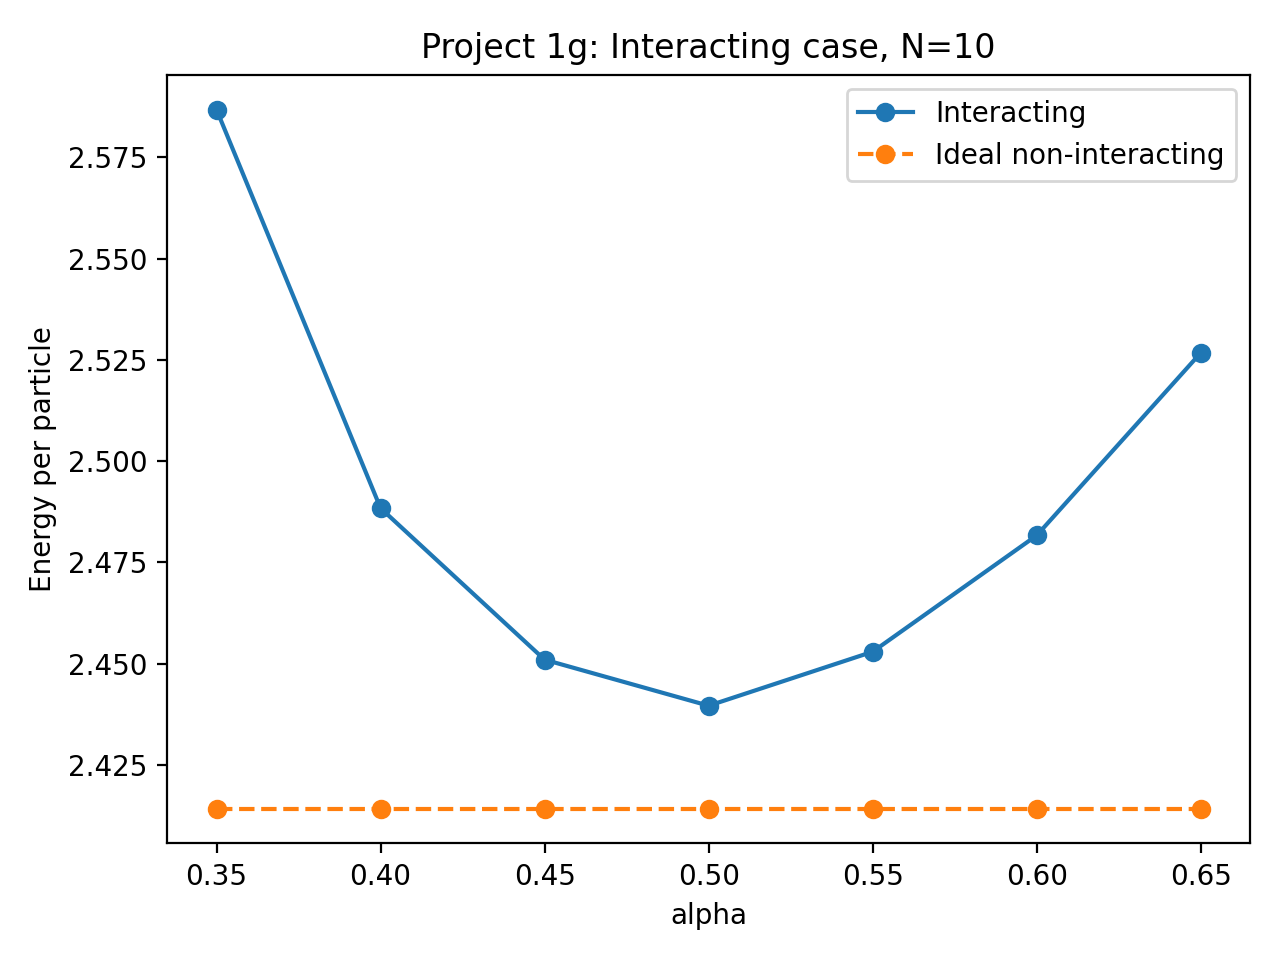
\includegraphics[width=\linewidth]{project1_g_energy_N10.png}\caption{$N=10$}\end{subfigure}
\begin{subfigure}{0.32\textwidth}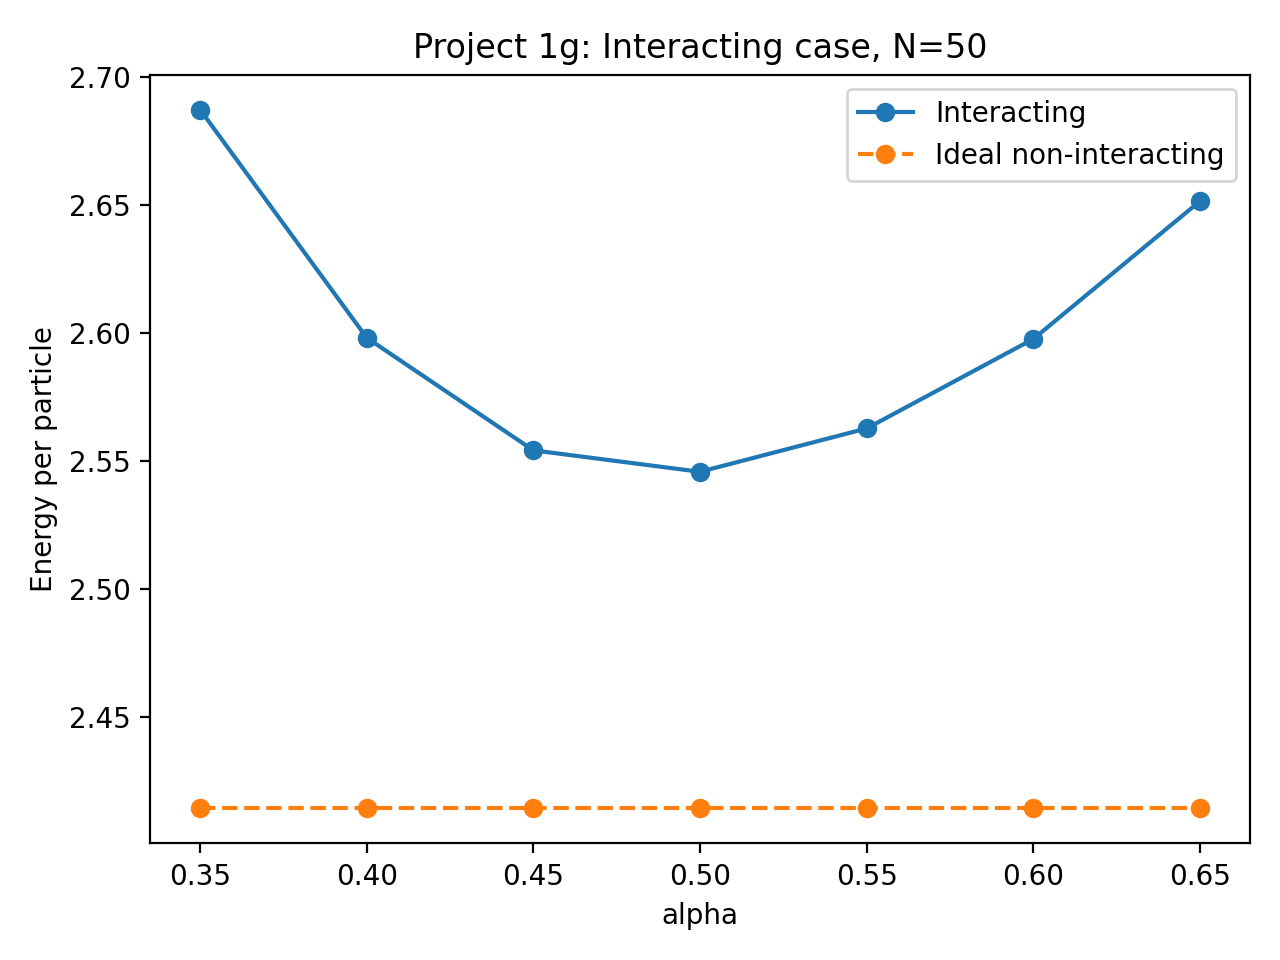
\includegraphics[width=\linewidth]{project1_g_energy_N50.png}\caption{$N=50$}\end{subfigure}
\begin{subfigure}{0.32\textwidth}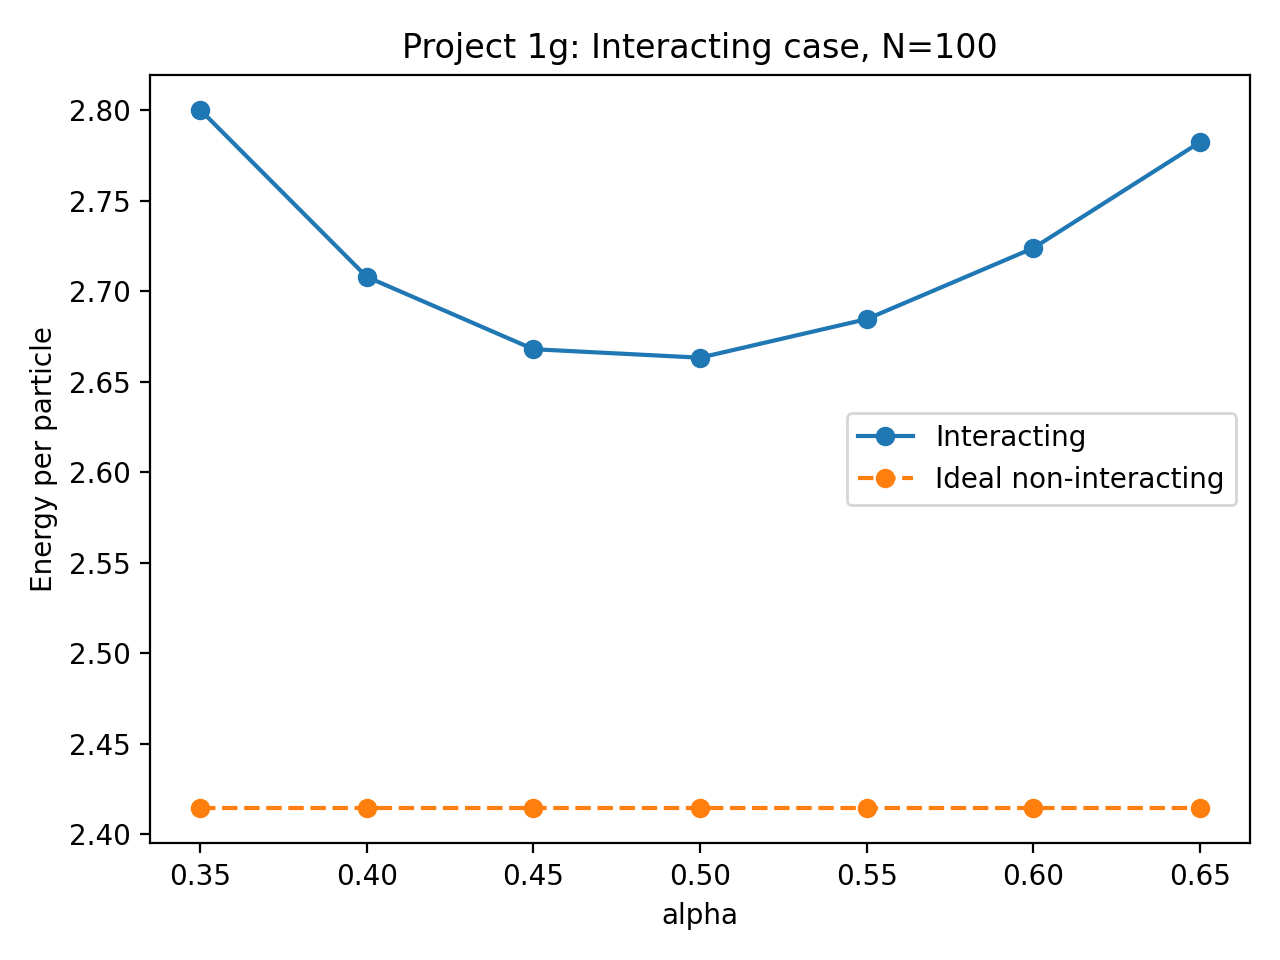
\includegraphics[width=\linewidth]{project1_g_energy_N100.png}\caption{$N=100$}\end{subfigure}
\caption{Project 1g interacting hard-core Bose gas in an anisotropic trap with $a/a_{\mathrm{ho}}=0.0043$ and $\beta=\gamma=2.82843$. The interacting energy is higher than the ideal non-interacting reference and increases with particle number.}
\label{fig:partg}
\end{figure*}

\begin{center}
\captionof{table}{Approximate minima from the interacting scans. The ideal reference is $E_0/N=2.414215$ for all three particle numbers.}
\label{tab:interacting-minima}
\setlength{\tabcolsep}{3pt}
\begin{tabular}{@{}cccc@{}}
\toprule
$N$ & best $\alpha$ & interacting $E/N$ & excess over ideal \\
\midrule
10  & 0.50 & 2.4396 & 0.0254\\
50  & 0.50 & 2.5457 & 0.1315\\
100 & 0.50 & 2.6633 & 0.2491\\
\bottomrule
\end{tabular}
\end{center}
The increasing excess energy is physically reasonable: for a fixed trap, more particles lead to stronger crowding and more frequent short-range correlations. This trend is consistent with the role of the hard-sphere Jastrow factor in earlier VMC studies of trapped bosons \cite{dubois2001}.

\subsection{One-body densities}

Figure~\ref{fig:parth} compares the one-body density with and without the hard-sphere Jastrow factor. The raw radial density $\rho(r)$ is largest near the origin and decays rapidly, as expected in a harmonic trap. The radial probability distribution $4\pi r^2\rho(r)$ is easier to interpret visually: it vanishes at the origin, peaks around $r\approx0.8$, and then decays.

The Jastrow and no-Jastrow curves are close. This is not surprising because the hard-core radius is very small compared with the oscillator length. The Jastrow factor acts mainly on short inter-particle distances, and its effect is therefore much stronger in pair-correlation observables than in the one-body density. Still, the small differences around the density peak indicate that correlations slightly redistribute the probability density.

\begin{figure*}[t]
\centering
\begin{subfigure}{0.47\textwidth}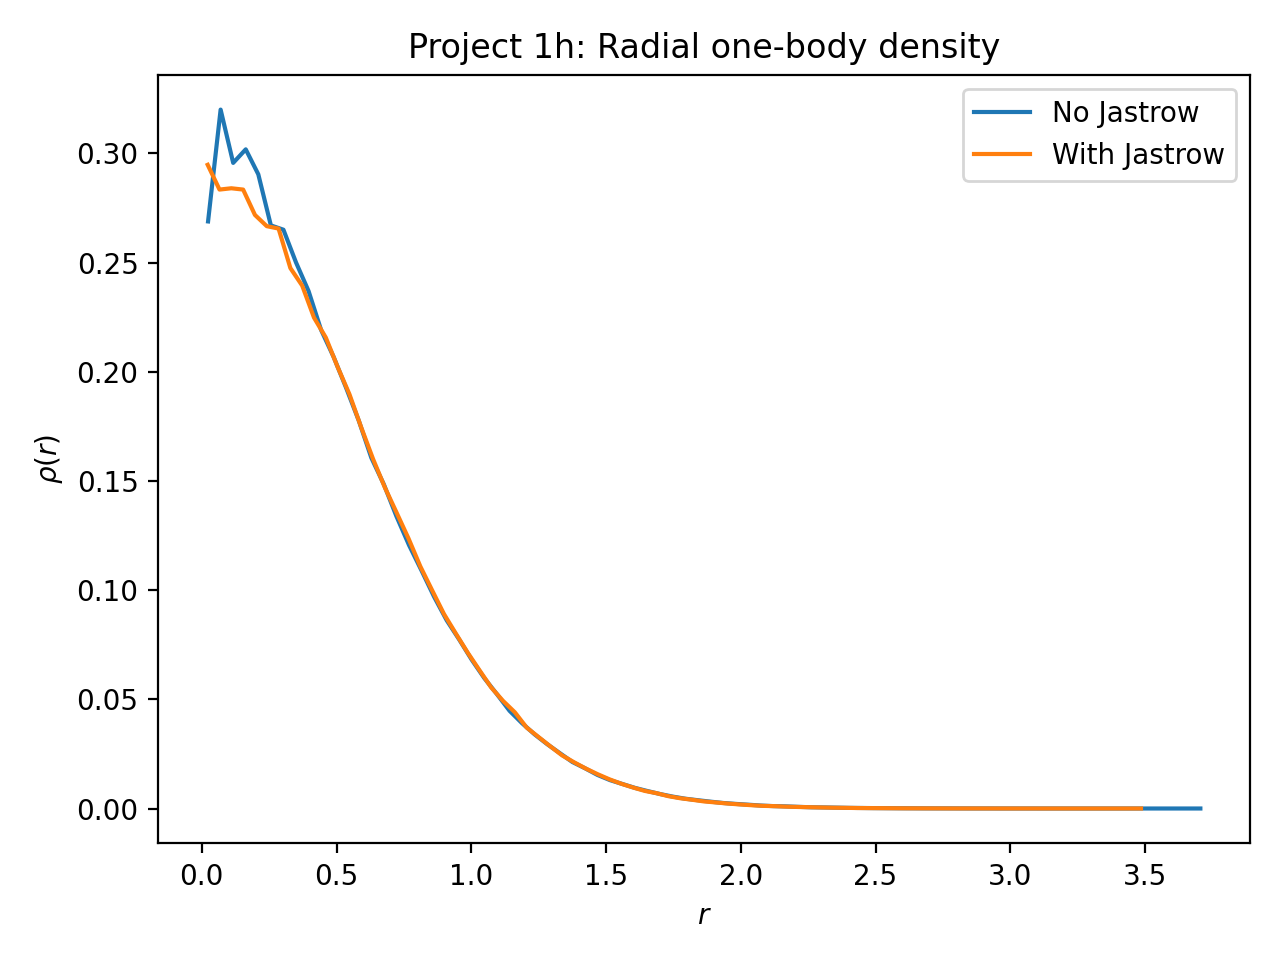
\includegraphics[width=\linewidth]{project1_h_radial_density.png}\caption{Radial density}\end{subfigure}
\begin{subfigure}{0.47\textwidth}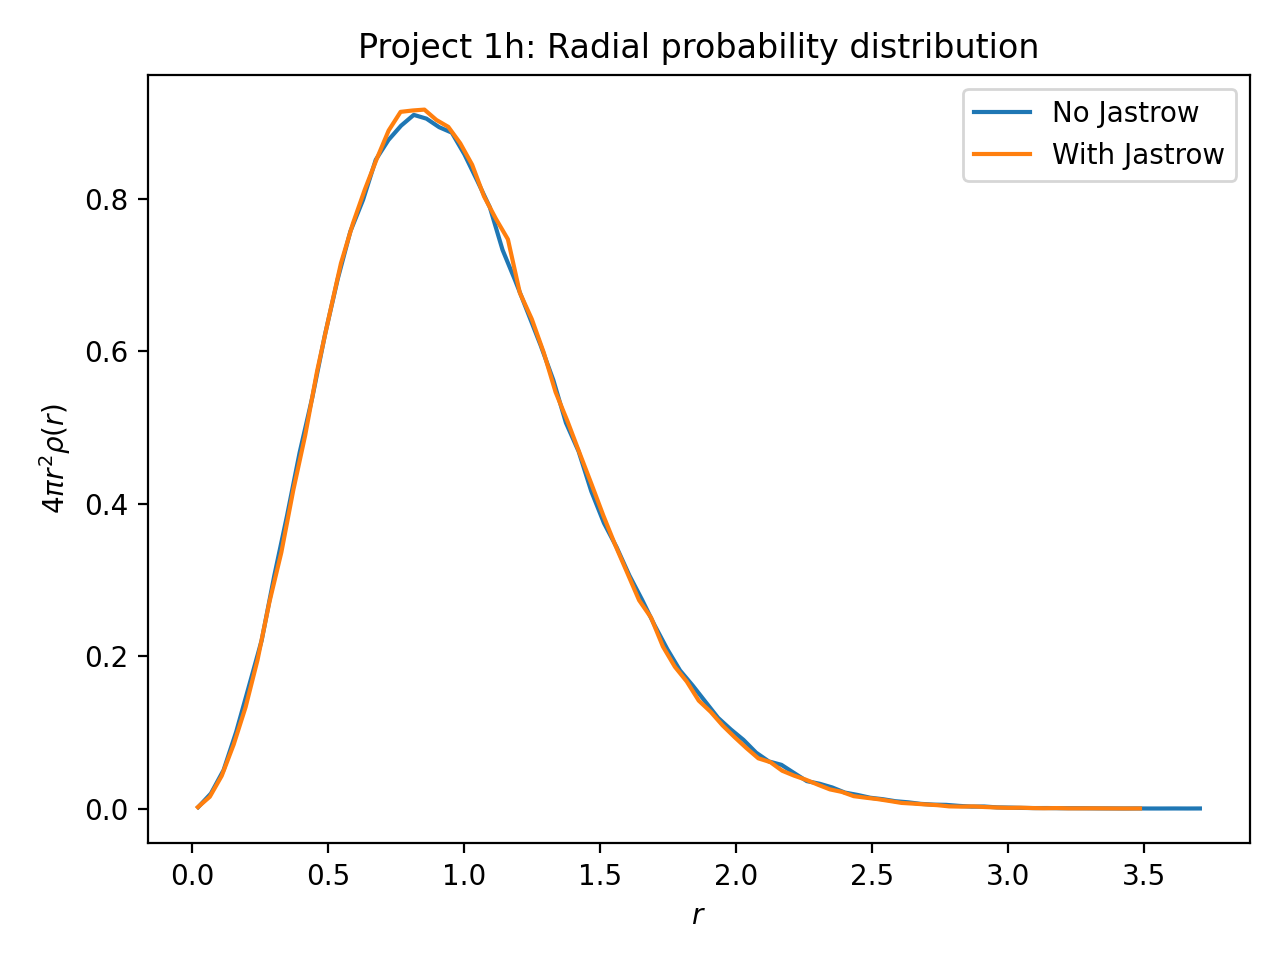
\includegraphics[width=\linewidth]{project1_h_radial_probability.png}\caption{Radial probability distribution}\end{subfigure}
\caption{Project 1h one-body density with and without the hard-sphere Jastrow factor. The direct one-body effect of the short-range correlation is small for $a/a_{\mathrm{ho}}=0.0043$, but the correlated and uncorrelated curves are not exactly identical.}
\label{fig:parth}
\end{figure*}

\clearpage
\section{Conclusions and perspectives}\label{sec:conclusion}

The VMC implementation reproduces the analytical non-interacting harmonic-oscillator benchmarks in one, two, and three dimensions. This validates the analytical local energy, drift force, Metropolis sampling, and result-writing pipeline. The brute-force Metropolis scans correctly identify the variational minimum at $\alpha=0.5$, and importance sampling gives the same exact result for the exact trial wave function. For a non-optimal trial function, the importance-sampling estimates fluctuate around the analytical variational energy, as they should.

The optimization part initially required care because too large a learning rate caused the parameter to jump between the imposed bounds. With a smaller learning rate, the optimization converged smoothly to $\alpha=0.5$ and $E=150$ for $N=100$ in three dimensions. This illustrates why optimization algorithms must be validated on analytically solvable cases before being trusted for interacting systems.

The hard-core interacting calculations show the expected qualitative behavior: the repulsive Jastrow factor raises the energy above the ideal trapped-gas reference, and the excess energy per particle increases with particle number. The optimal Gaussian parameter remains close to $\alpha=0.5$ for the parameters studied. The one-body density changes only weakly when the Jastrow factor is included, which is reasonable because the hard-core radius is very small in oscillator units.

The main limitations are computational cost and statistical resolution. The large-$N$ interacting runs are slow in pure Python, and the blocking analysis would benefit from longer time series. Future improvements include vectorizing more of the interacting local energy, adding parallel sampling, computing pair-correlation functions, and performing a more detailed quantitative comparison with the published VMC/DMC benchmarks of trapped hard-sphere bosons.

\appendix
\section{Reproducibility and code usage}\label{app:reproducibility}

The main production commands used for the report were:
\begin{lstlisting}
python scripts/run_project1_b.py --cycles 50000 --burn-in 5000
python scripts/run_project1_c.py --n-particles 100 --cycles 50000 --burn-in 5000
python scripts/run_project1_c.py --n-particles 100 --alpha 0.45 \
    --cycles 20000 --burn-in 2000 \
    --output data/results/project1_c_importance_alpha045.csv
python scripts/run_project1_d.py --n-particles 100 --dimensions 3 \
    --initial-alpha 0.7 --learning-rate 0.001 \
    --iterations 20 --cycles 30000 --burn-in 3000
python scripts/run_project1_e.py --n-particles 100 --alpha 0.45 \
    --cycles 50000 --burn-in 5000 \
    --blocking-output data/results/project1_e_blocking_alpha045.csv \
    --summary-output data/results/project1_e_summary_alpha045.csv
python scripts/run_project1_g.py --cycles 30000 --burn-in 3000
python scripts/run_project1_h.py --n-particles 10 --cycles 50000 \
    --burn-in 5000 --alpha 0.5
\end{lstlisting}

The tests are run with
\begin{lstlisting}
pytest -q
\end{lstlisting}
and passed with 25 tests before the final plots were generated.

\section{Comments on numerical reliability}

The exact non-interacting cases provide the strongest validation. At $\alpha=0.5$ the local energy has zero variance, so these results should not be interpreted as typical Monte Carlo uncertainties. The $\alpha=0.45$ runs are more useful for checking statistical analysis because they have finite variance. For the blocking plot, the error estimate should be chosen from the region where the curve is approximately stable; the final few points can fluctuate because too few blocks remain.

For the interacting case, the hard-core boundary condition makes the local energy more expensive and increases the importance of good sampling. The results should therefore be interpreted primarily through trends and consistency checks unless longer production runs and direct literature benchmarks are added.

\begin{thebibliography}{9}

\bibitem{dubois2001}
J. L. DuBois and H. R. Glyde, "Bose--Einstein condensation in trapped bosons: A variational Monte Carlo analysis," \emph{Physical Review A} \textbf{63}, 023602 (2001).

\bibitem{nilsen2005}
J. K. Nilsen, J. Mur-Petit, M. Guilleumas, M. Hjorth-Jensen, and A. Polls, "Vortices in atomic Bose--Einstein condensates in the large-gas-parameter region," \emph{Physical Review A} \textbf{71}, 053610 (2005).

\bibitem{metropolis1953}
N. Metropolis, A. W. Rosenbluth, M. N. Rosenbluth, A. H. Teller, and E. Teller, "Equation of State Calculations by Fast Computing Machines," \emph{Journal of Chemical Physics} \textbf{21}, 1087--1092 (1953).

\bibitem{umrigar1993}
C. J. Umrigar, M. P. Nightingale, and K. J. Runge, "A diffusion Monte Carlo algorithm with very small time-step errors," \emph{Journal of Chemical Physics} \textbf{99}, 2865--2890 (1993).

\bibitem{flyvbjerg1989}
H. Flyvbjerg and H. G. Petersen, "Error estimates on averages of correlated data," \emph{Journal of Chemical Physics} \textbf{91}, 461--466 (1989).

\bibitem{foulkes2001}
W. M. C. Foulkes, L. Mitas, R. J. Needs, and G. Rajagopal, "Quantum Monte Carlo simulations of solids," \emph{Reviews of Modern Physics} \textbf{73}, 33--83 (2001).

\end{thebibliography}

\end{document}
